\section{Jet Reconstruction and Selection}
\label{ch:JetReconstruction}

\subsection{Tracks}
\label{sec:TrackSelection}

Tracks are required to have a minimum \pT of 150 MeV/c. Tracks with constituent \pT up to 200 GeV/$c$ are accepted, the limit of which is constrained by ALICE track resolution. Tracks with a \pT larger than 100 GeV/$c$ have a significantly worse \pT resolution. Figure~\ref{fig:ptresolution} shows the \pT resolution for \pp and \pPb collisions for events using the jet triggers, which cover the high momentum range in this measurement. This is accounted for in the systematic uncertainties by varying the maximum track \pT. The tracking efficiency falls sharply in the forward and backward region, and thus, tracks are required to fall in the pseudorapidity range $|\eta| < 0.9$. Hybrid tracks are used for this analysis, meaning high quality (global) tracks that have at least one hit in the SPD combined with complimentary tracks that include the primary-vertex and do not fail a refit of the track when including hits from the ITS.

\begin{figure}[hbt!]
    \centering
    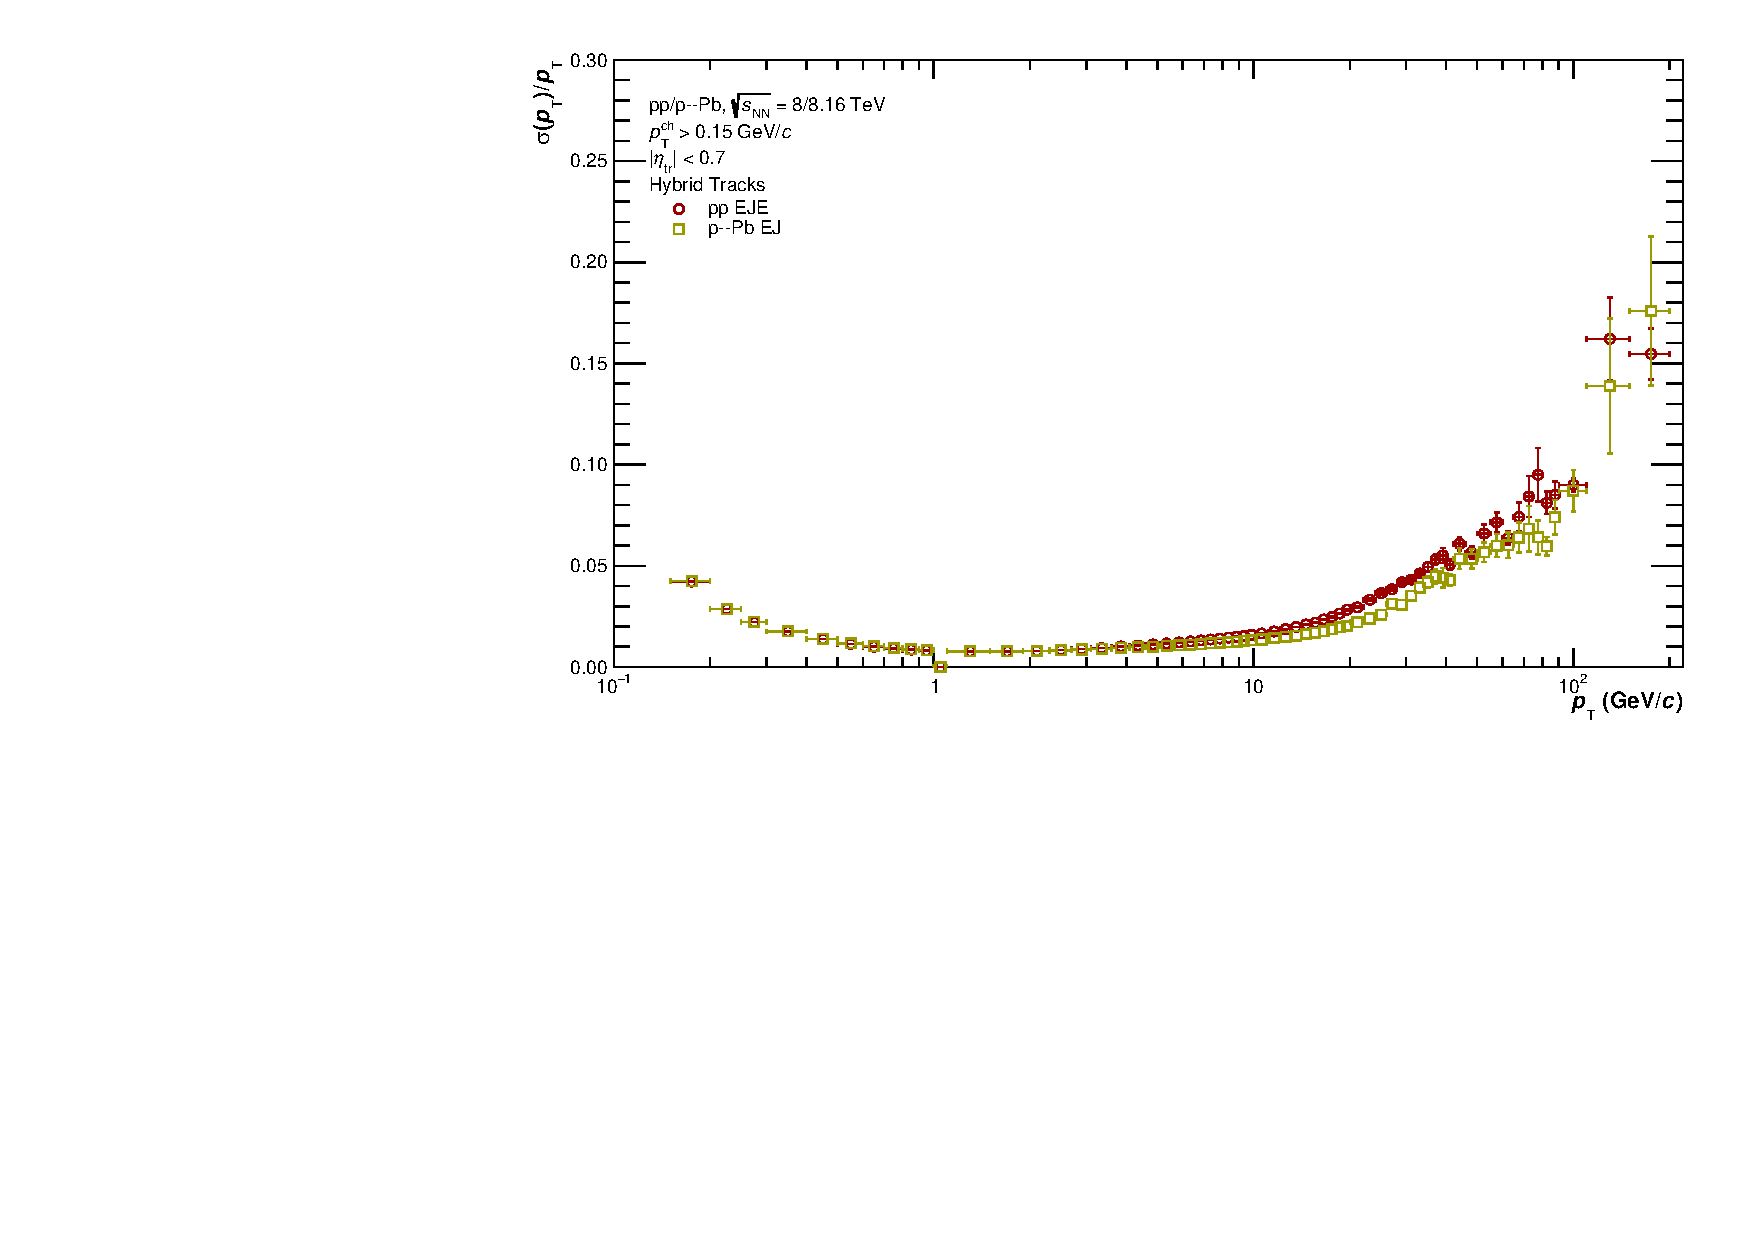
\includegraphics[width=\textwidth]{figures/TrackingQA/PtResolution/PtRes_ppVSpPb.pdf}
    \caption{Transverse momentum resolution for tracks in \pp and \pPb collisions in EMCal jet triggered events.}
    \label{fig:ptresolution}
\end{figure}

\subsection{EMCal Clusters}
\label{sec:ClusterSelection}

When a particle hits the EMCal, it will induce a shower that is primarily contained in one EMCal cell, but spreads out to adjacent cells. These cells must be combined through a process called clusterization in order to reconstruct the full particle energy. The primary cell must pass a specified seed threshold, and then cells are added to the cluster until no adjacent cell above the specified cell threshold remains.

EMCal clusters reconstructed with the v3-clusterizer algorithm are required to have a minimum energy of 300 MeV. Additional corrections for clusters reconstructed in the EMCal can be found in the recent EMCal performance paper~~\cite{EMCalPerformance2022}. Particles from multiple bunch crossings can be recorded in the same event. This includes event pileup and slowly propagating particles such as slow neutrons. In order to remove clusters from different bunch crossings within the EMCal integration window, only energy deposits within [-30,+35] ns for \pp and [-50,+50] ns for \pPb with respect to the measured bunch crossing time are considered. These are the cuts used within the GA group, and the same was followed here. Cluster energy measured before the event cannot be from the event, given a finite resolution, and are concluded to be from beam-gas interactions or event pileup. Cluster energy measured after the event arises from beam-gas interactions or slower particles that take longer to propagate through the detectors. 

In order to avoid double counting of energy deposited by charged particles in the EMCal, the contribution from all tracks matched to clusters is estimated and subtracted from the cluster energy using momentum-dependent track matching. Exotic clusters, i.e clusters with a very high percentage of energy deposited in a single cell due to a high-energy particle hitting one of the avalanche photodiodes, are removed from the analysis. EMCal clusters are accepted up to an energy of 200 GeV. Above this energy, the response of the EMCal is substantially non-linear and is not well understood (see Figure~\ref{fig:emcal_testbeam}). Clusters are corrected for non-linearity using the final corrections stated in the recent EMCal performance paper \cite{EMCalPerformance2022}. This corresponds to kTestBeamShaper and kTestBeamFinalMC for data and monte carlo, respectively. The maximum cluster energy is also varied in the systematic uncertainties to account for this effect. The EMCal trigger cluster yields for all three triggers in \pp collisions are shown in Figure~\ref{fig:triggerClusters_pp}, given for jet resolution parameter $R$ = 0.2. The same is shown for \pPb collisions in Figure~\ref{fig:triggerClusters_pPb}. The cluster and jet yields from each trigger are at different scales due to the downscaling of the minimum bias, EMC7, and EJ2 triggers to different degrees in order to allow trigger time for the EMCal triggers to record rare events such as jets. This scaling must be corrected before the results from different event triggers are combined. As the integrated luminosity is independent of the probe, the scaling can be determined solely based on the EMCal clusters regardless of the jet reconstruction algorithm.


\begin{figure}[hbt!]
    \centering
    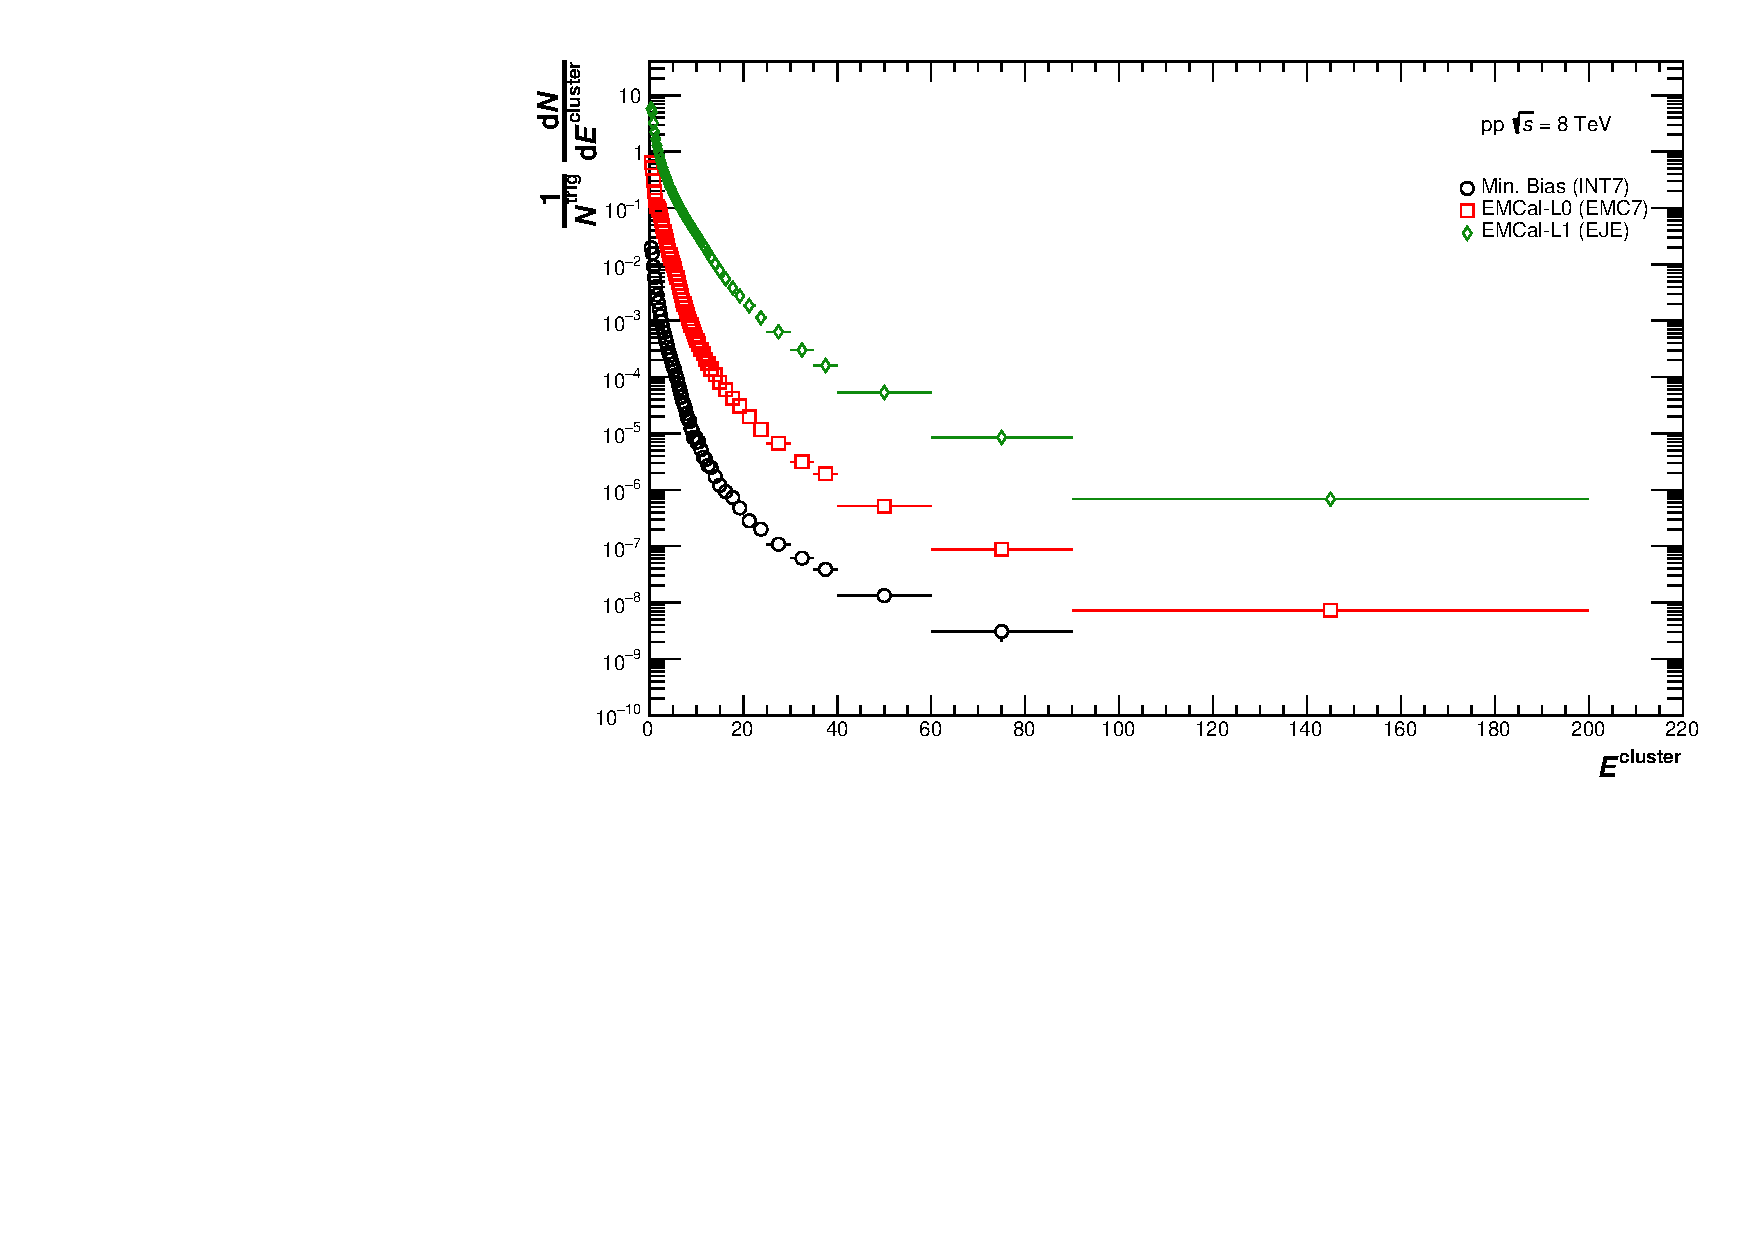
\includegraphics[width=15cm]{figures/TriggerClusters/clusters_R02.pdf}
    \caption{Trigger cluster yields for the INT7, EMC7, and EJE triggers in \pp. Scaling by the rejection factor is required in order for the spectra to overlap.}
    \label{fig:triggerClusters_pp}
\end{figure}

\begin{figure}[hbt!]
    \centering
    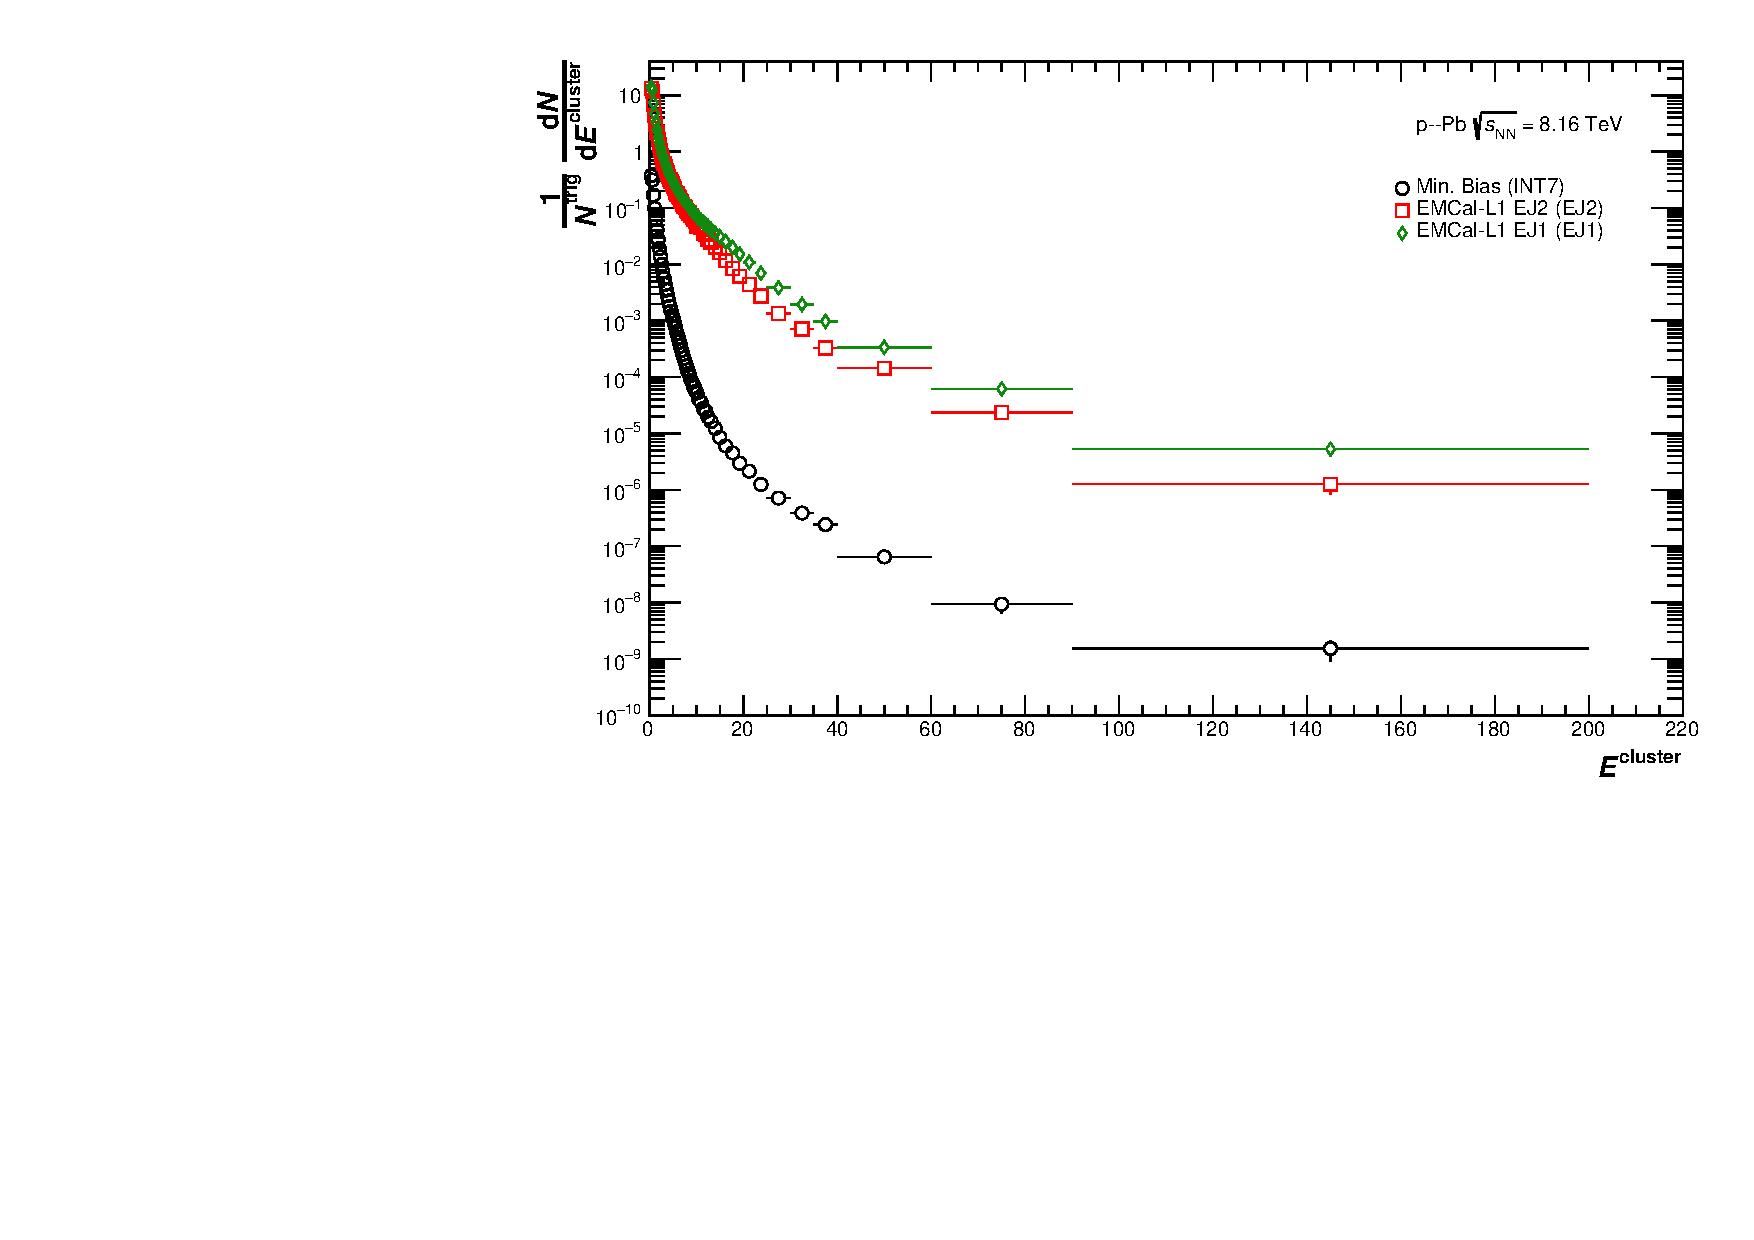
\includegraphics[width=15cm]{figures/pPbFigures/TriggerClusters/clusters_R02.pdf}
    \caption{Trigger cluster yields for the INT7, EJ2, and EJ1 triggers in \pPb. Scaling by the rejection factor or by the trigger luminosity is required in order for the spectra to overlap.}
    \label{fig:triggerClusters_pPb}
\end{figure}

\subsection{Jets}
\label{sec:JetSelection}

Jets are reconstructed using the anti-k$_T$ algorithm~\cite{Cacciari:2008gp} under the \pT-scheme using the FastJet~\cite{Cacciari:2011ma} package. These methods for track, cluster and jet selection were also used in previous measurements, such as in Ref.~\cite{anaNoteMFasel}, and are standard for jet analyses in ALICE. Jets are required to be fully contained within the EMCal acceptance and have a minimum \pT of 10 GeV/$c$. Jets are reconstructed with a resolution parameter defined as $R = \sqrt{(\Delta\eta)^2 + (\Delta\phi)^2}$. The area of the jet must pass the cut $A_{jet} > 0.6\pi R^2$ to suppress background, where $\pi R^2$ is the area of a jet cone with resolution parameter $R$. After all cuts have been applied, the average number of both tracks and clusters in a jet is around 3 to 4 tracks/clusters in the low \pT range of the measurement and around 8 to 9 tracks/clusters in the high \pT range of the measurement. These numbers hold for both \pp and \pPb collisions.

The selected jet \pT ranges for \pp collisions are 20 to 240 GeV/$c$ for jet radii R = 0.2 to 0.5 and 20 to 160 GeV/$c$ for R = 0.6, where the statistics in the highest bins limit the extent of the spectrum. For \pPb collisions, the range for R = 0.2 to 0.4 is 20 to 240 GeV/$c$, while R = 0.5 is limited to 20 to 120 GeV/$c$. R = 0.6 is not included in the \pPb analysis due to a lack of statistics for the entire \pT range. The jet \pT ranges along with trigger patch sizes and thresholds can be found in Table~\ref{tab:trigger_ranges}.


\begin{table}[hbt!]
    \centering
    \caption{EMCal trigger thresholds, patch sizes, and momentum ranges for different triggers in \pp and \pPb collisions. The lower value in brackets refers to the limit at large jet radii.}
    \begin{tabular}{  m{2cm} | m{3.2cm} | m{3.2cm} | m{3.2cm} | m{3.2cm}  }
        \hline
        System & Trigger Name & Momentum Range (GeV/$c$) & Patch Size (cells) & Threshold (GeV) \\
        \hline
        \pp & INT7 & 20--30 & & \\
            & EMC7 & 30--50 & 4x4 & 2.067 \\
            & EJE & 50--[240/160] & 32x32 & 15.6 \\
        \hline
        \pPb & INT7 & 20--30 & & \\
             & EJ2 & 30--50 & 32x32 & 18 \\
             & EJ1 & 50--[240/120] & 32x32 & 23 \\
        \hline
    \end{tabular}
    \label{tab:trigger_ranges}
\end{table}

% For thesis presentation only:
\iffalse
\begin{table}[hbt!]
    \centering
    \begin{tabular}{  m{2cm} | m{3.2cm} | m{3.2cm} | m{3.2cm} | m{3.2cm}  }
        \hline
        System & Trigger Name & Momentum Range (GeV/$c$) & Threshold (GeV), Patch Size (cells) & $\mathscr{L}_{\text{int}}  (\text{nb}^{-1})$ \\
        \hline
        \pp   & INT7 (Min Bias) & \textbf{20}--30 & & 1.03 \\
        8 TeV & EMC7 (EMCal $\gamma$) & 30--60 & 2.076, 4x4 & 41.4 \\
              & EJE (EMCal Jet) & 60--\textbf{[240/160]} & 15.6, 32x32 & 8.75 \\
        \hline
        \pPb     & INT7 (Min Bias) & \textbf{20}--30 & & 7.35$\times 10^{-3}$ \\
        8.16 TeV & EJ2 (EMCal Jet) & 30--50 & 18, 32x32 & 6.51$\times 10^{-2}$ \\
                 & EJ1 (EMCal Jet) & 50--\textbf{[240/120]} & 23, 32x32 & 1.34 \\
        \hline
    \end{tabular}
\end{table}
\fi

\subsection{Bias of the EMCal Trigger}
\label{sec:EMCTriggerBias}

The EMCal measures all interacting particles, including photons, leptons, and hadrons. Photons can originate directly from the primary vertex, but come primarily from the decay of neutral hadrons such as the $\pi^0$ meson. Hadrons that interact directly with the calorimeter include those which leave minimal ionization energy and those which interact hadronically and leave a partial shower. Since the matched tracks are subtracted off if they are matched to an EMCal cluster, a large portion of the remaining particles are photons. For this reason, it is referred to as the neutral energy fraction (NEF), although the contribution from neutral hadrons interacting directly with the EMCal is small. The neutral energy fraction is the fraction of energy from the track + EMCal cluster composite object coming from the cluster.

The EMCal triggers are used to measure high energy jet events. As the trigger selects jets based on the amount of energy deposited in the calorimeter, it introduces a bias on the jets that vanishes only at higher \pT. Figure~\ref{fig:NEF} shows the comparison of the distribution of the neutral energy fraction for \pp jets in minimum bias and triggered events for various bins in jet \pT for R = 0.2 jets. The distributions are compared to the neutral energy fraction distributions calculated using a PYTHIA8 simulation. For other radii and equivalent plots in \pPb, see Appendix~\ref{sec:appendixTriggerBiaspPb}. Figure~\ref{fig:meanNEF_pp} shows the mean neutral energy fraction in \pp collisions for various jet resolution parameters, and Figure~\ref{fig:meanNEF_pPb} shows the same in \pPb collisions.

For the lowest jet \pT bins, the distributions show significant scale differences. At low \pT, jets in EMCal triggered events are dominated by the neutral component. Jets are required to deposit enough energy in the EMCal to pass the trigger. For jets with a given energy in the low momentum regime close to the trigger threshold, only those that deposit a larger fraction of their energy in the EMCal will pass the threshold. At lower \pT in minimum bias events, an effect is seen from the different track and cluster \pT cutoffs of 150 MeV and 300 MeV. As jet \pT decreases, it is more likely to find jets which are dominated by charged particles as opposed to calorimeter clusters, since the cutoff for tracks is lower. Only for jets with \pT larger than 30 GeV/$c$ for EMC7 and 60 GeV/$c$ for EJE, the distributions for the triggers start overlapping with the distribution in minimum bias events. For \pPb, this occurs at 30 GeV for the EJ2 trigger and 50 GeV for the EJ1 trigger. These effects can also be seen in figure 100 of the 2022 EMCal Performance paper \cite{EMCalPerformance}.

The effect from the trigger bias is also shown in Figure~\ref{fig:trigger_ratios}, the \pT dependence of the jet yield ratio of EMC7/INT7 and EJE/EMC7, which fluctuates with \pT until a plateau is reached at approximately 30 GeV for EMC7 and approximately 60 GeV for EJE. At this point, the trigger approaches maximum efficiency, and the bias is minimized. Jets are selected in triggered events only in this low-bias region. 


\begin{figure}[hbt!]
    \centering
    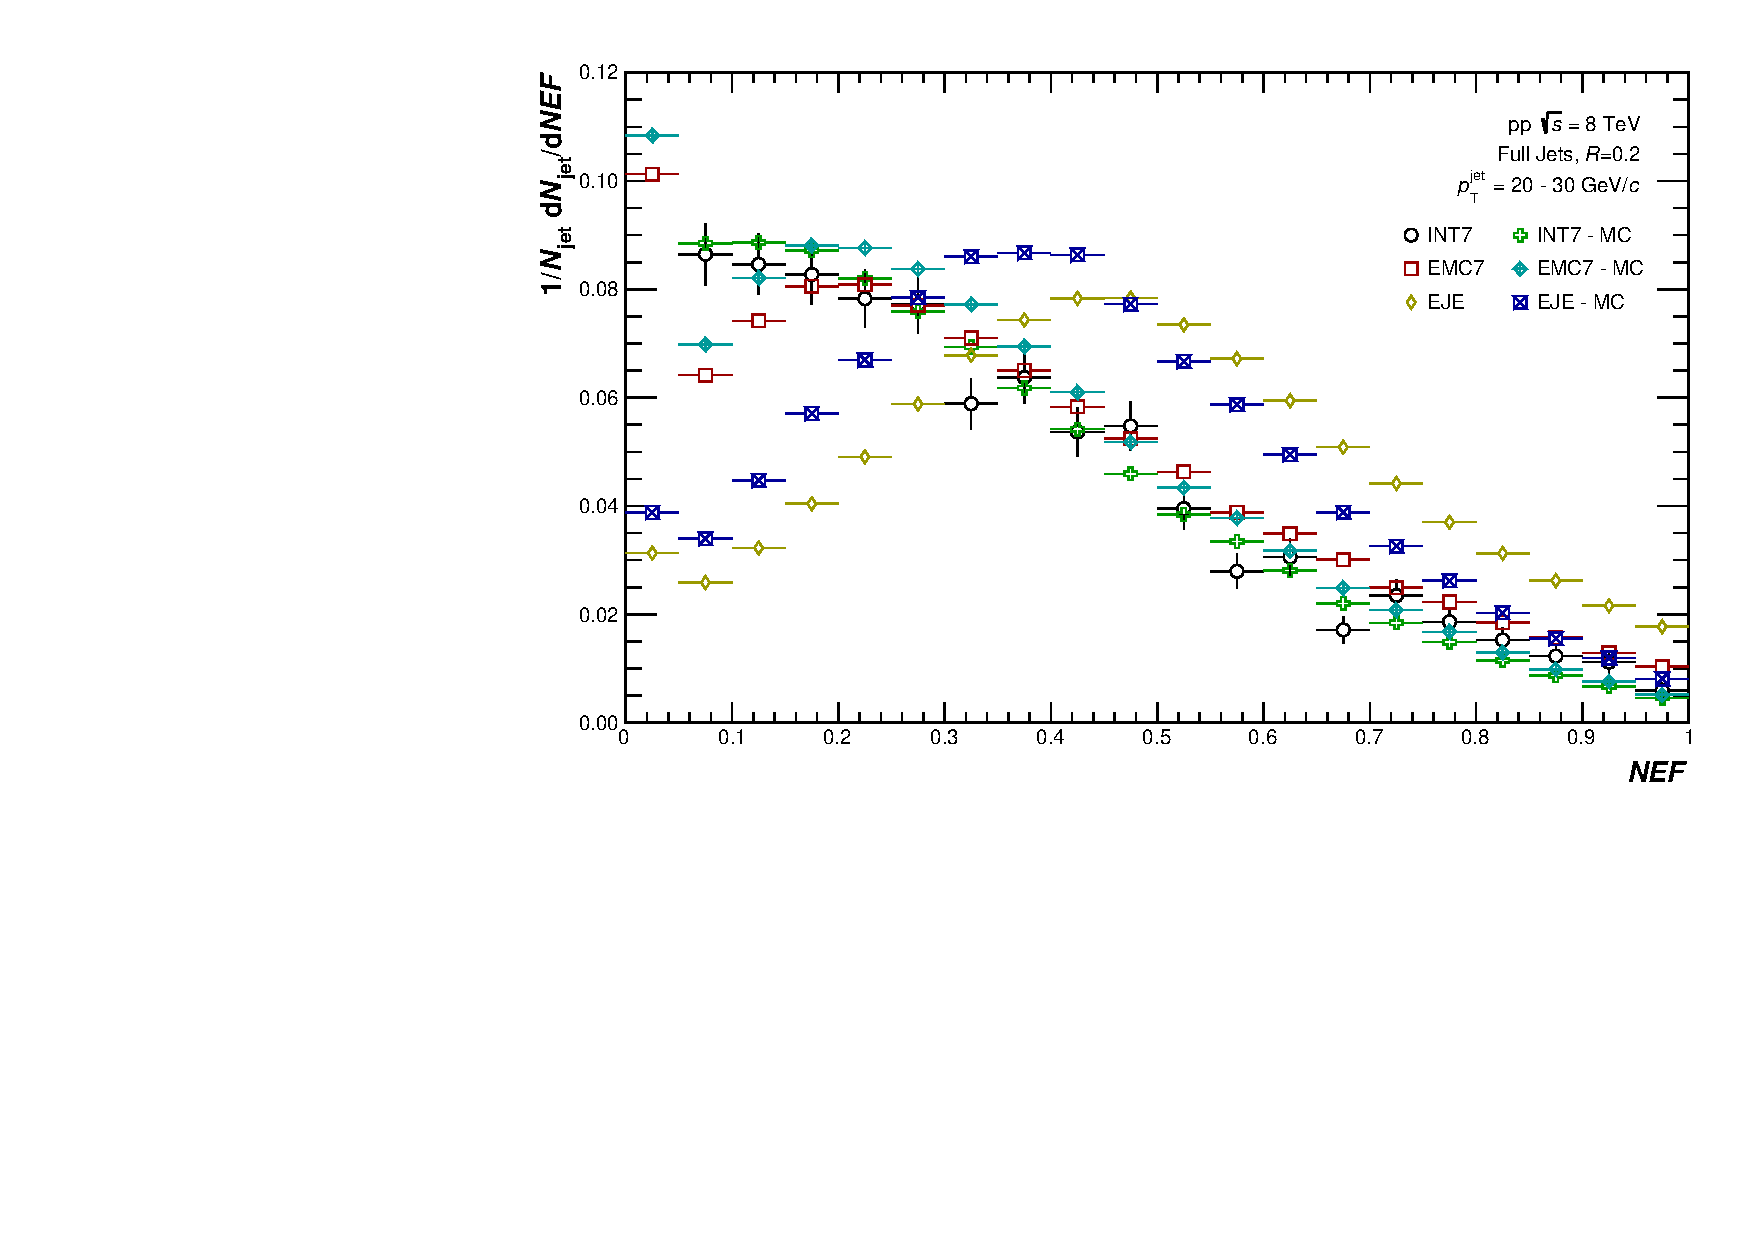
\includegraphics[width=0.49\textwidth]{figures/TriggerBias/NEF/All/hNEF_20-30GeV_R02.pdf}
    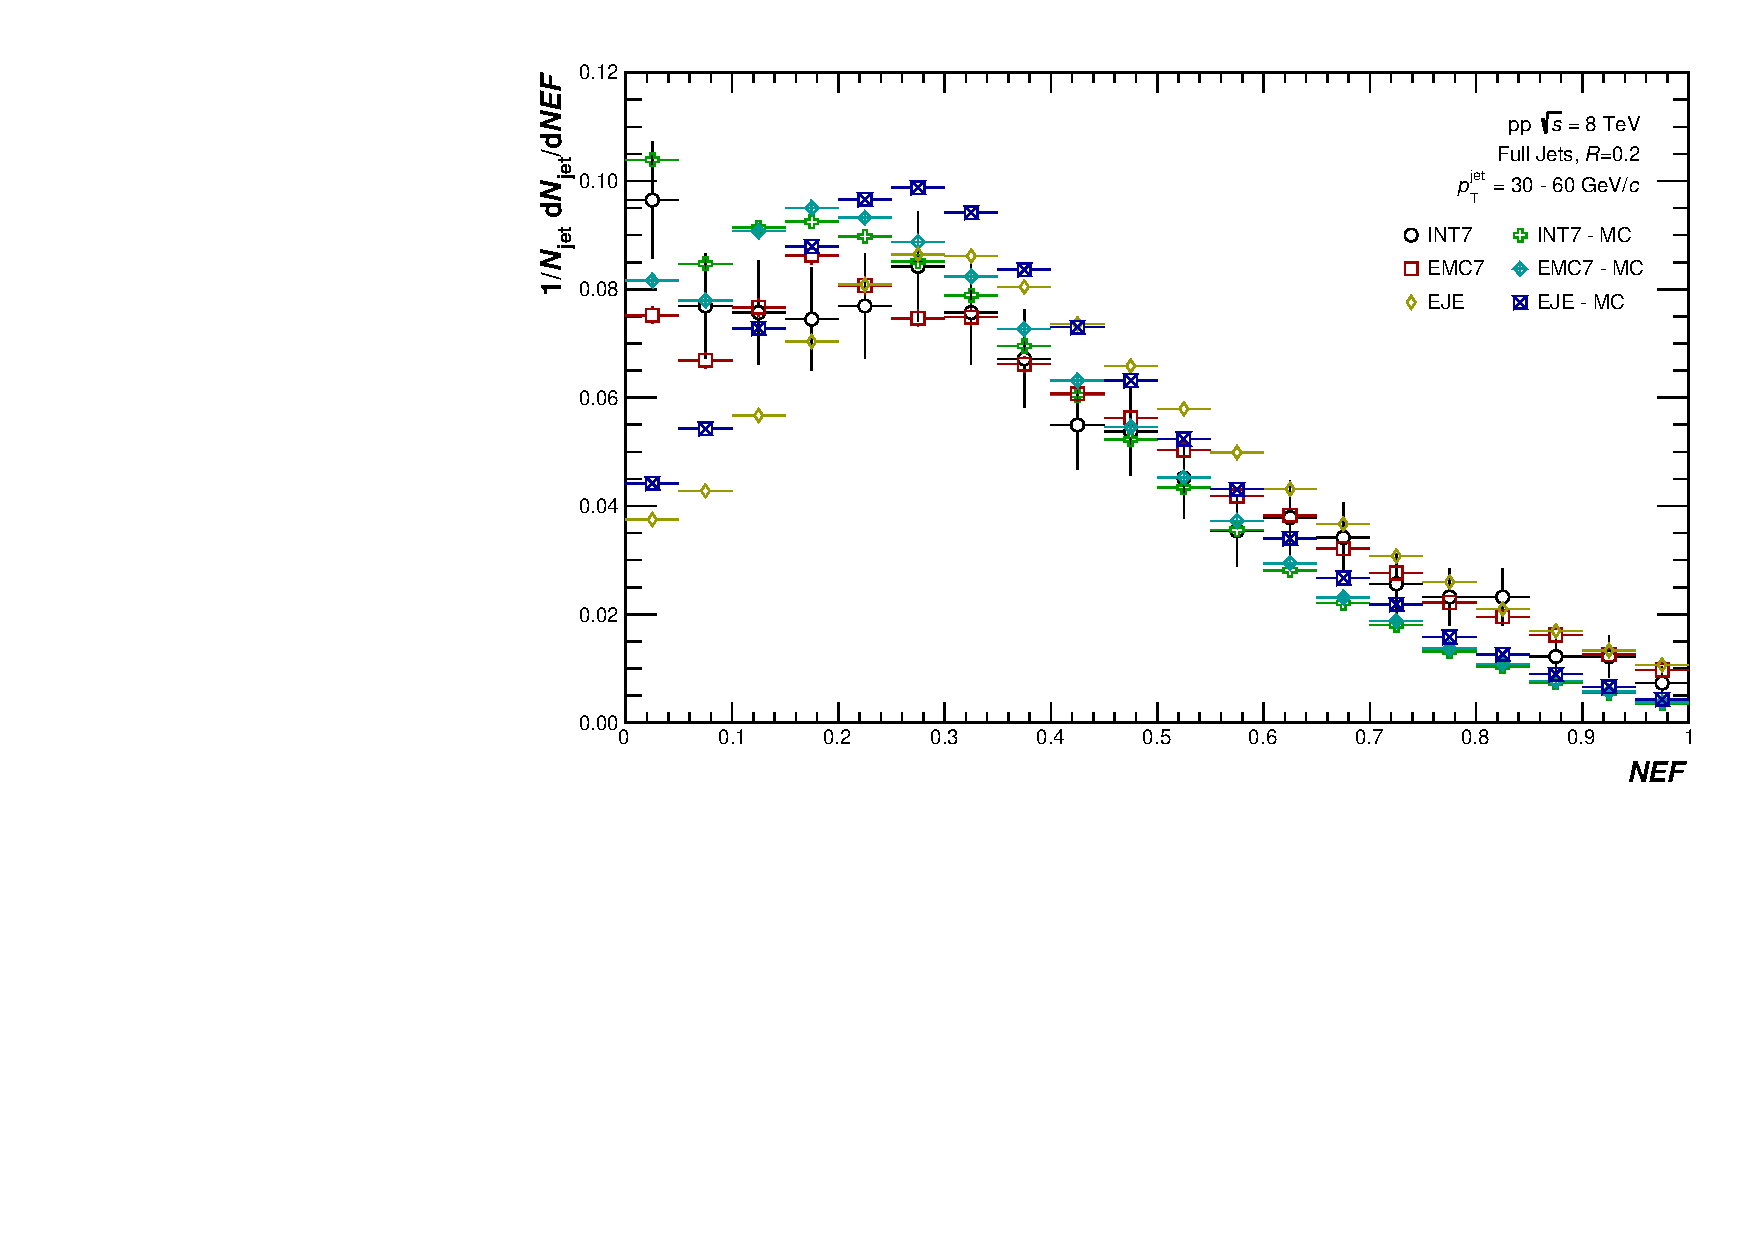
\includegraphics[width=0.49\textwidth]{figures/TriggerBias/NEF/All/hNEF_30-60GeV_R02.pdf}
    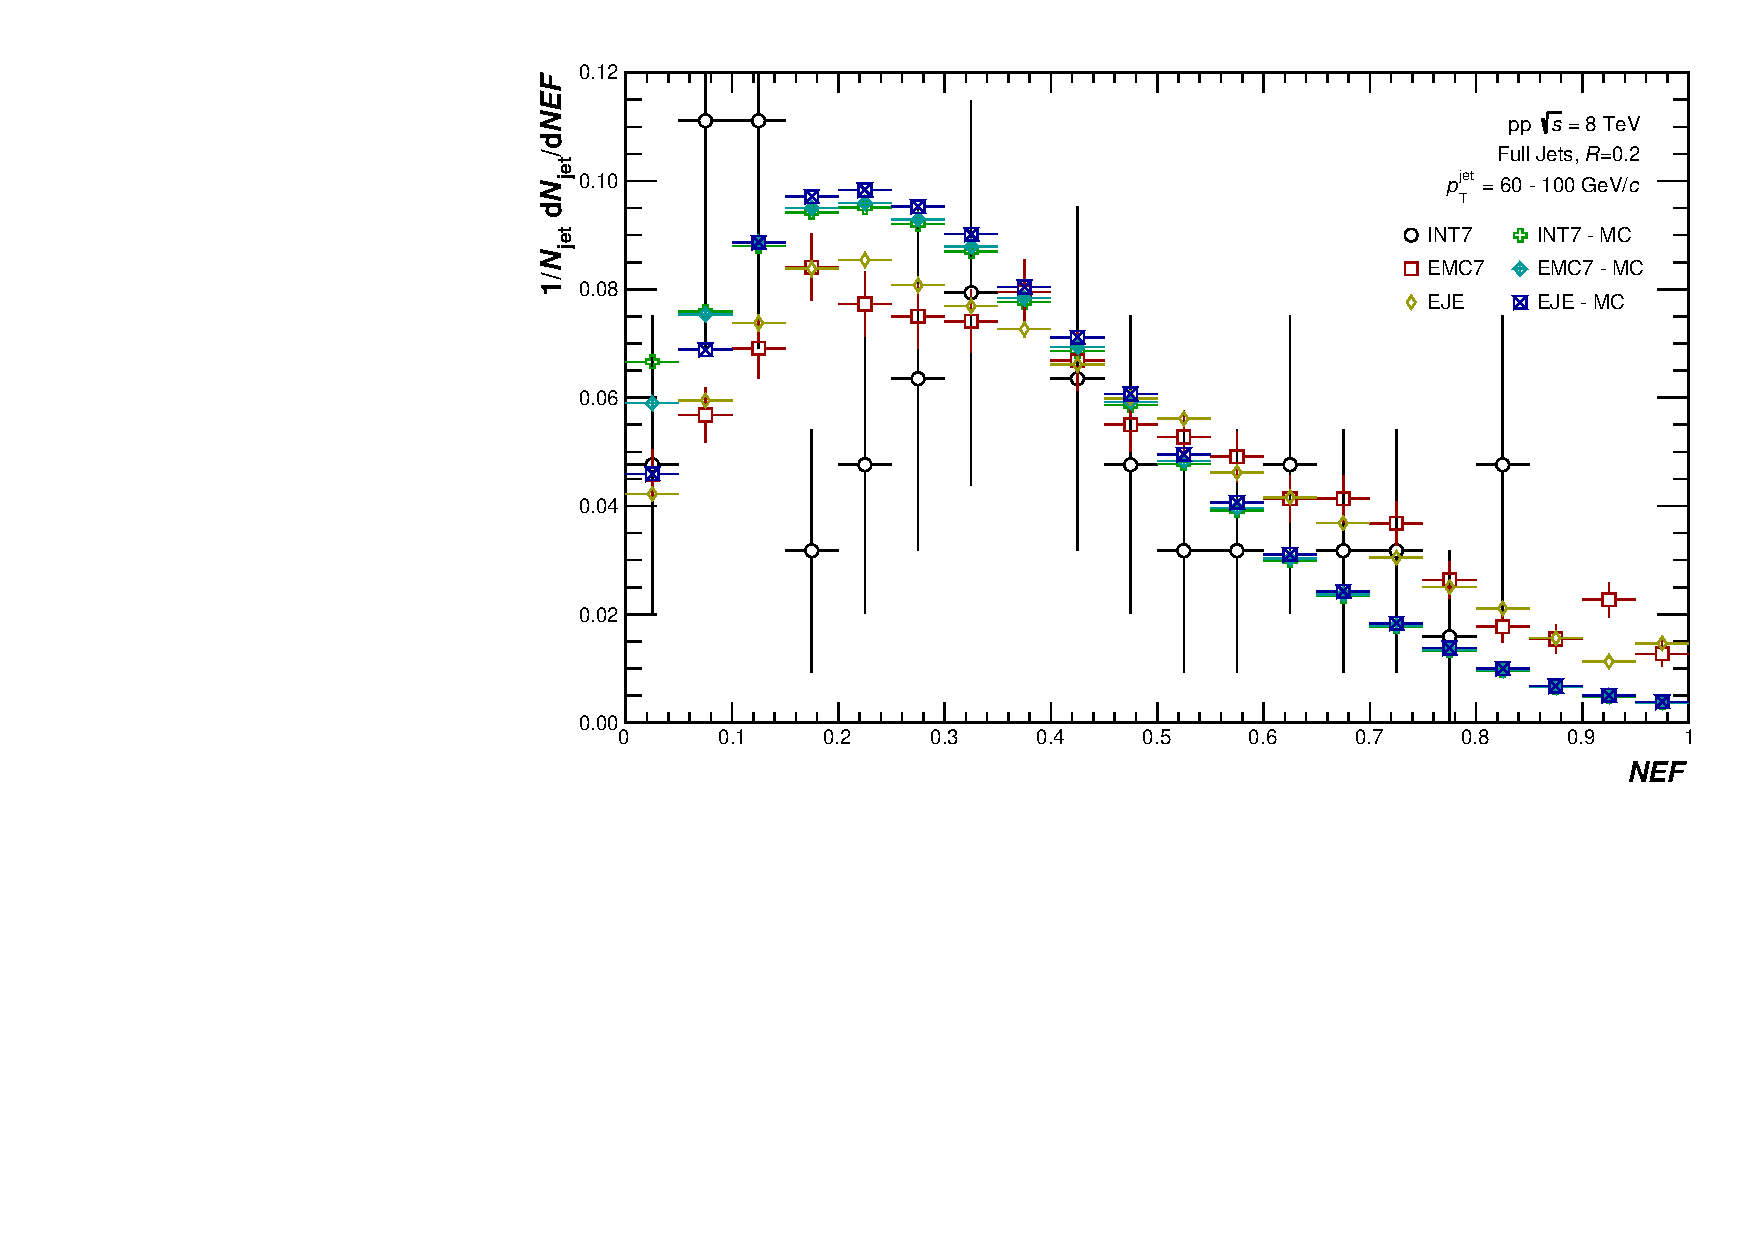
\includegraphics[width=0.49\textwidth]{figures/TriggerBias/NEF/All/hNEF_60-100GeV_R02.pdf}
    \caption{Probability distribution of the neutral energy fraction for jets in \pp collisions in data and PYTHIA8 found using the minimum bias and EMCal triggers for different bins in jet energy using R = 0.2 jets.}
    \label{fig:NEF}
\end{figure}

\begin{figure}[hbt!]
    \centering
    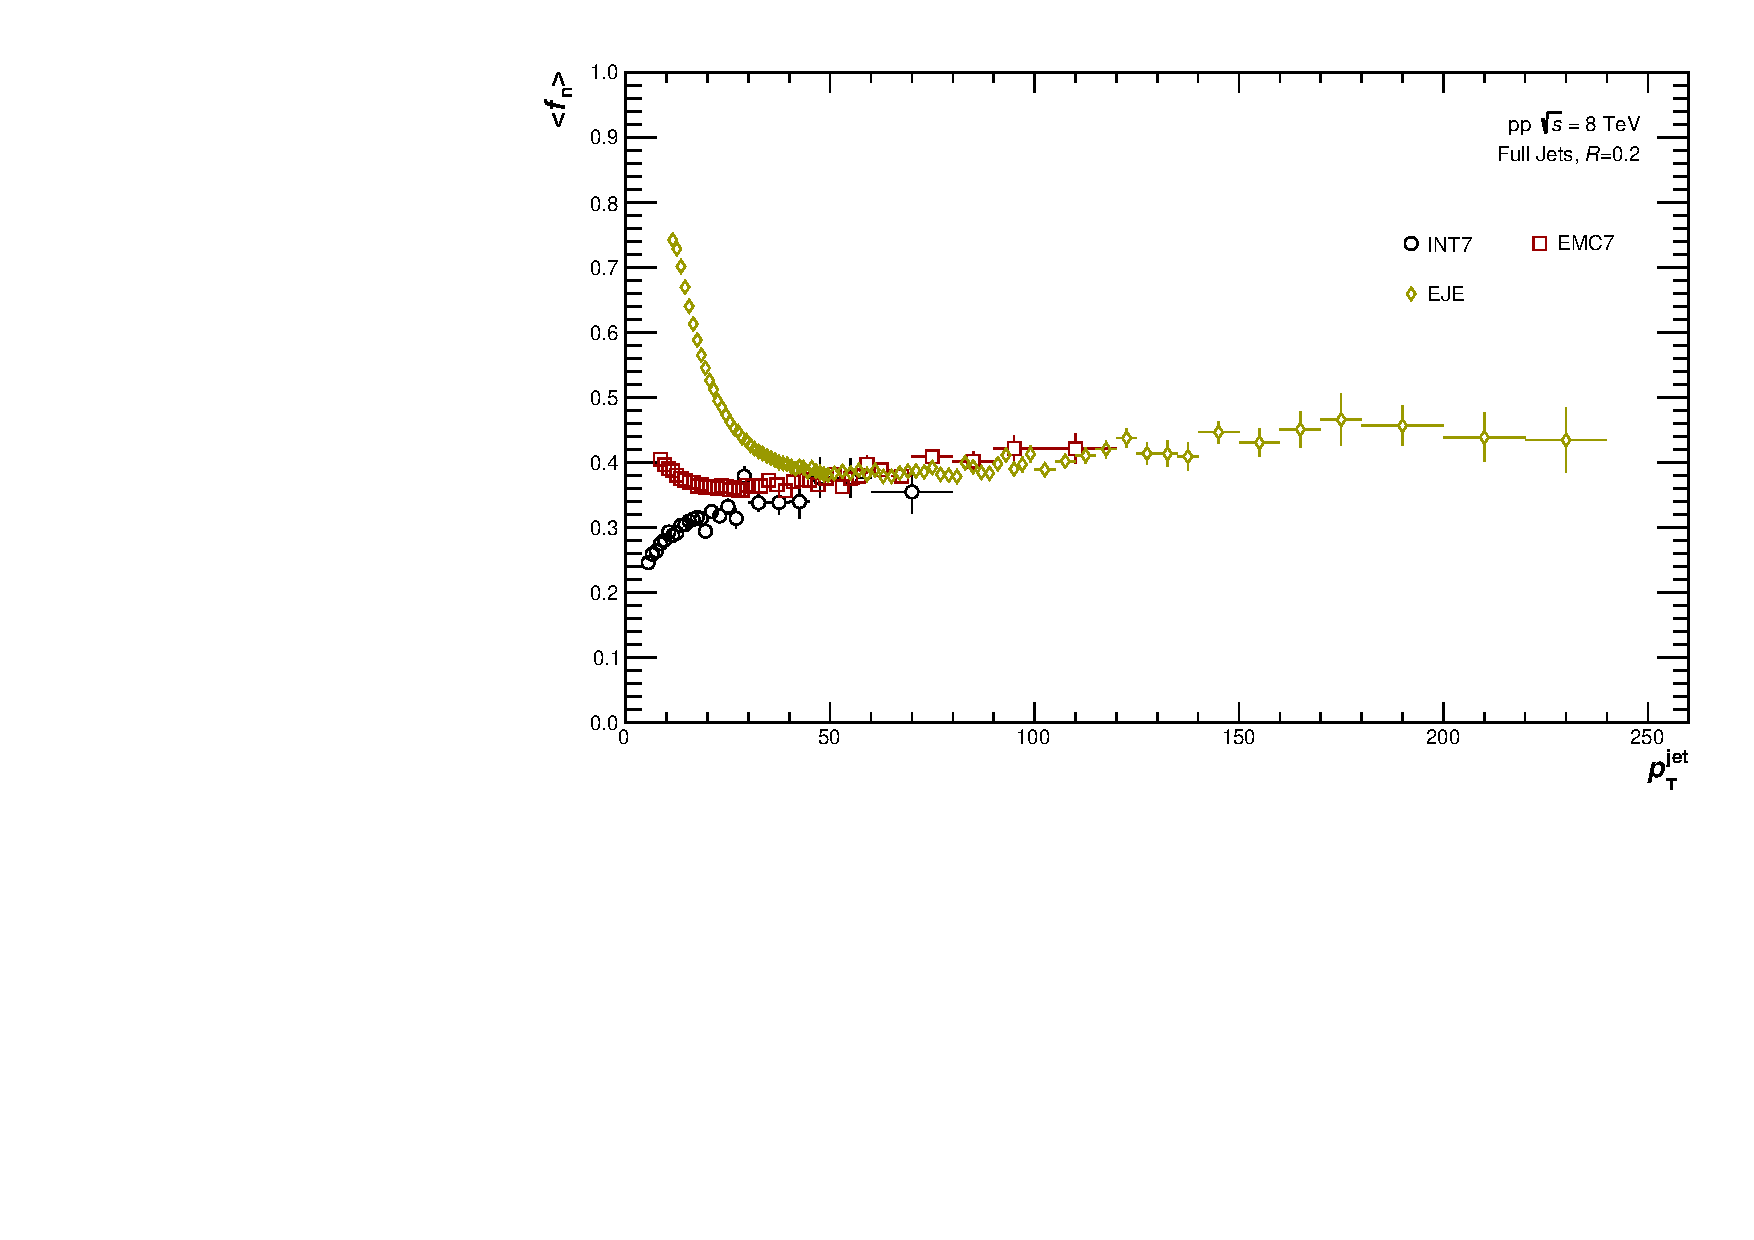
\includegraphics[width=0.49\textwidth]{figures/TriggerBias/NEF/All/mean_NEF_R02.pdf}
    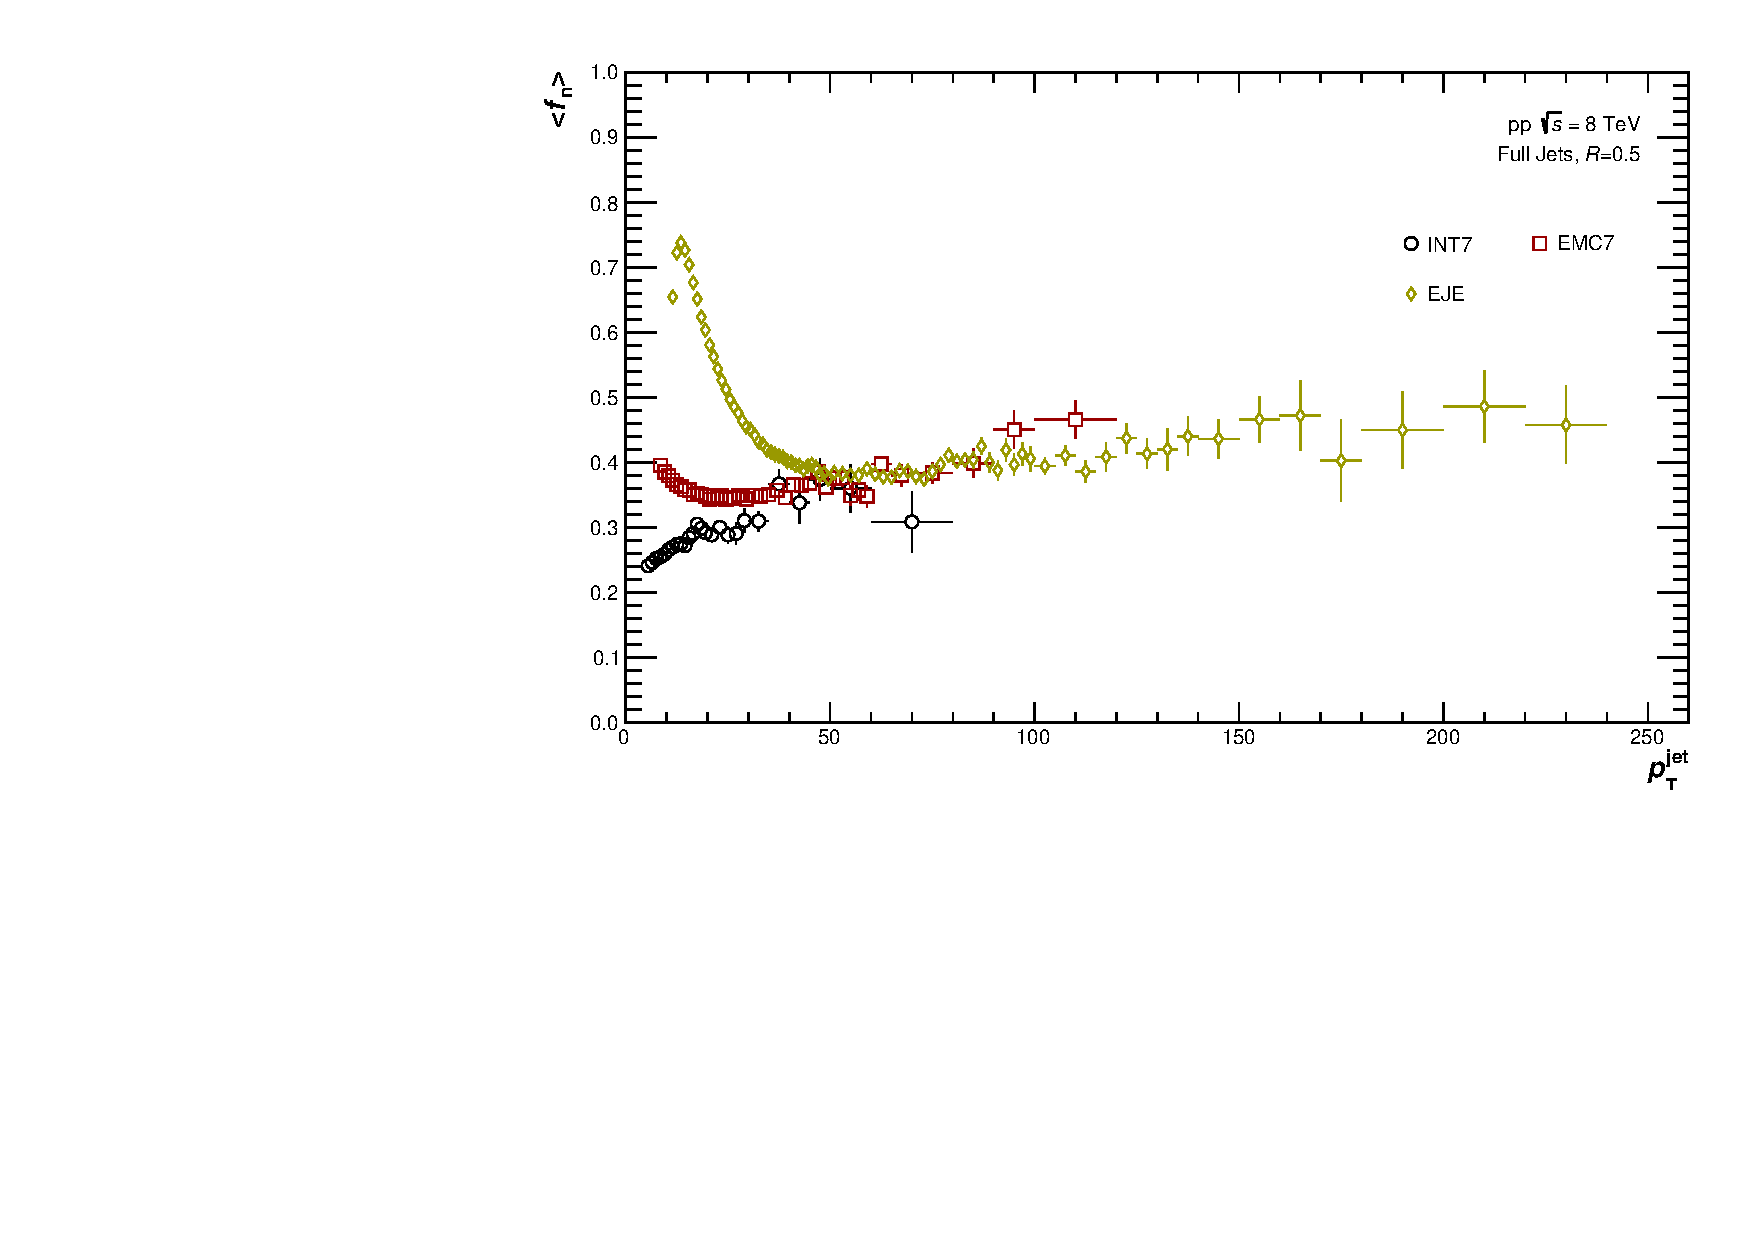
\includegraphics[width=0.49\textwidth]{figures/TriggerBias/NEF/All/mean_NEF_R05.pdf}
    \caption{Mean neutral energy fraction as a function of jet \pT for jets in \pp collisions for minimum bias and EMCal triggers, presented for various jet resolution parameters.}
    \label{fig:meanNEF_pp}
\end{figure}

\begin{figure}[hbt!]
    \centering
    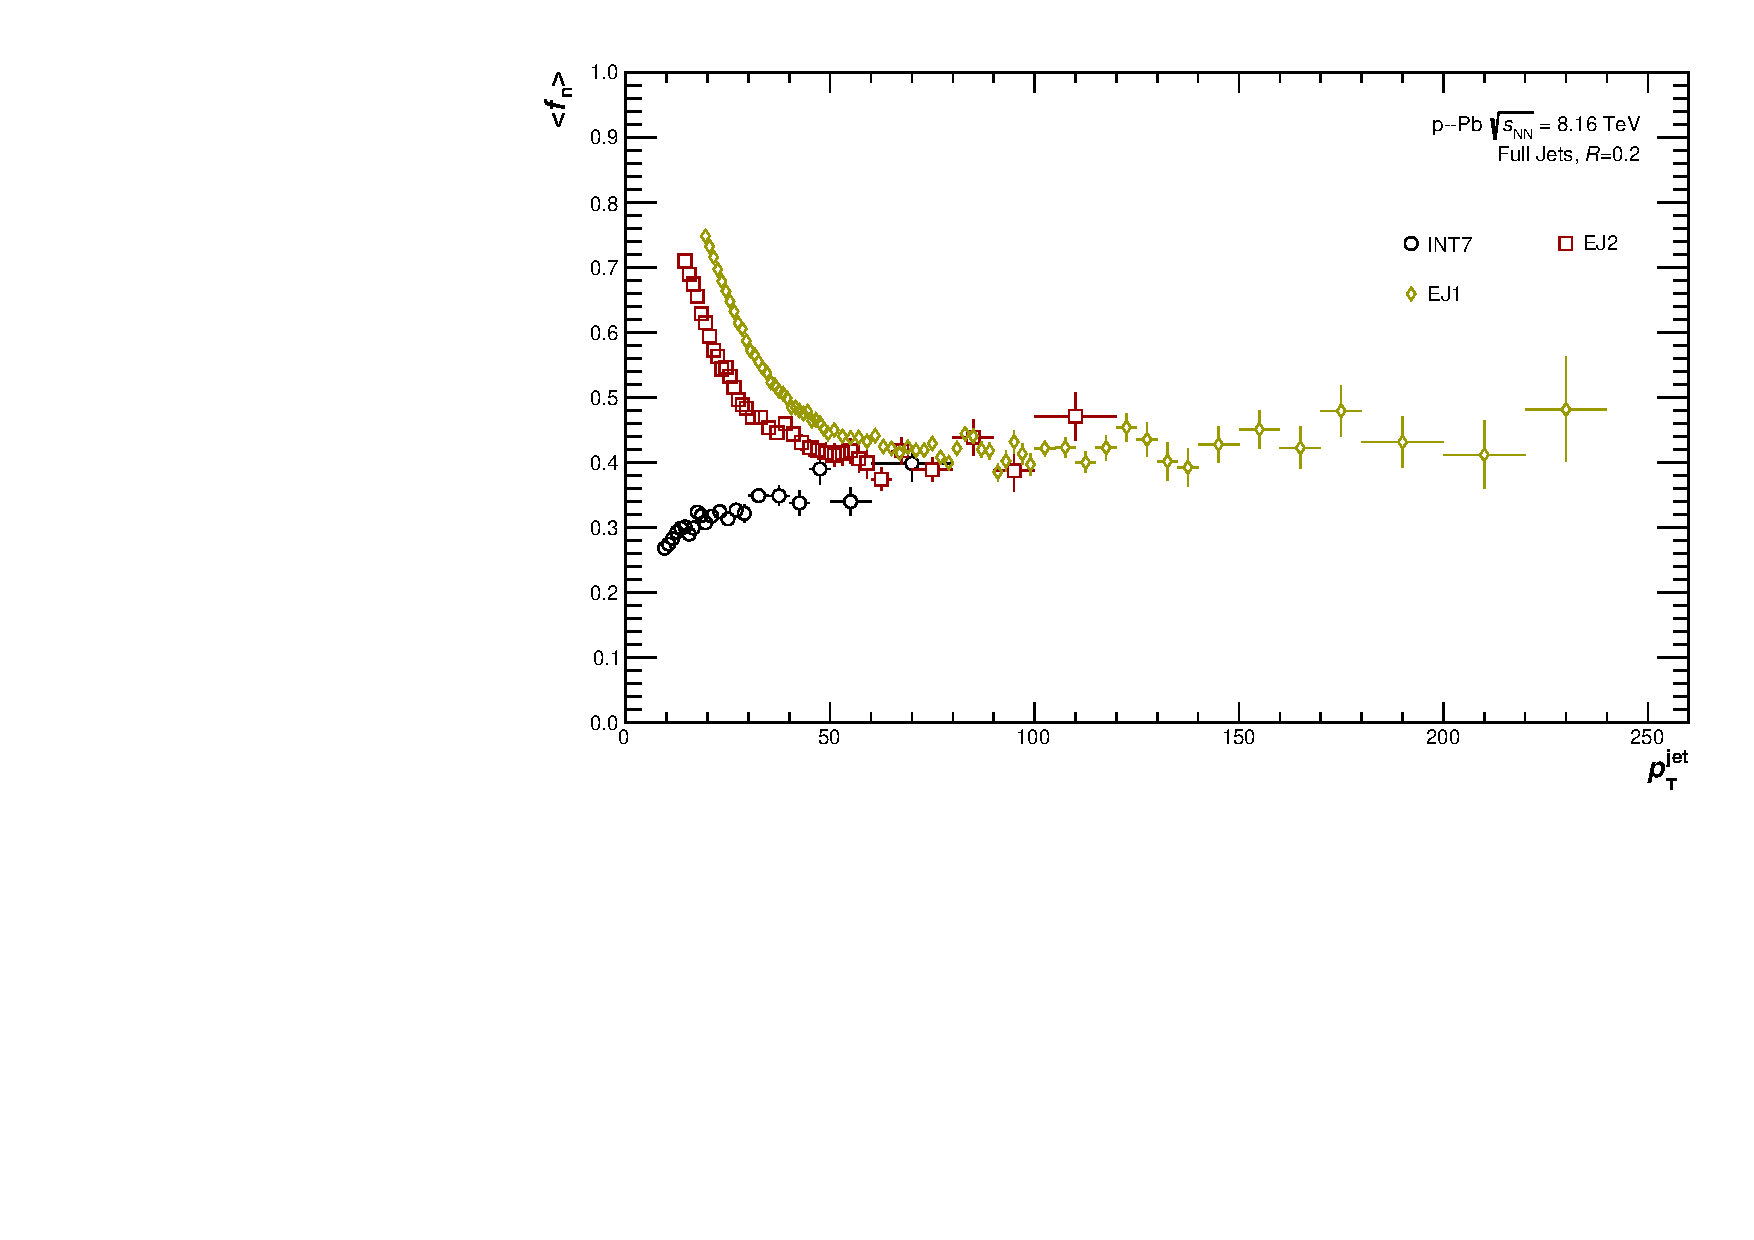
\includegraphics[width=0.49\textwidth]{figures/pPbFigures/TriggerBias/NEF/All/mean_NEF_R02.pdf}
    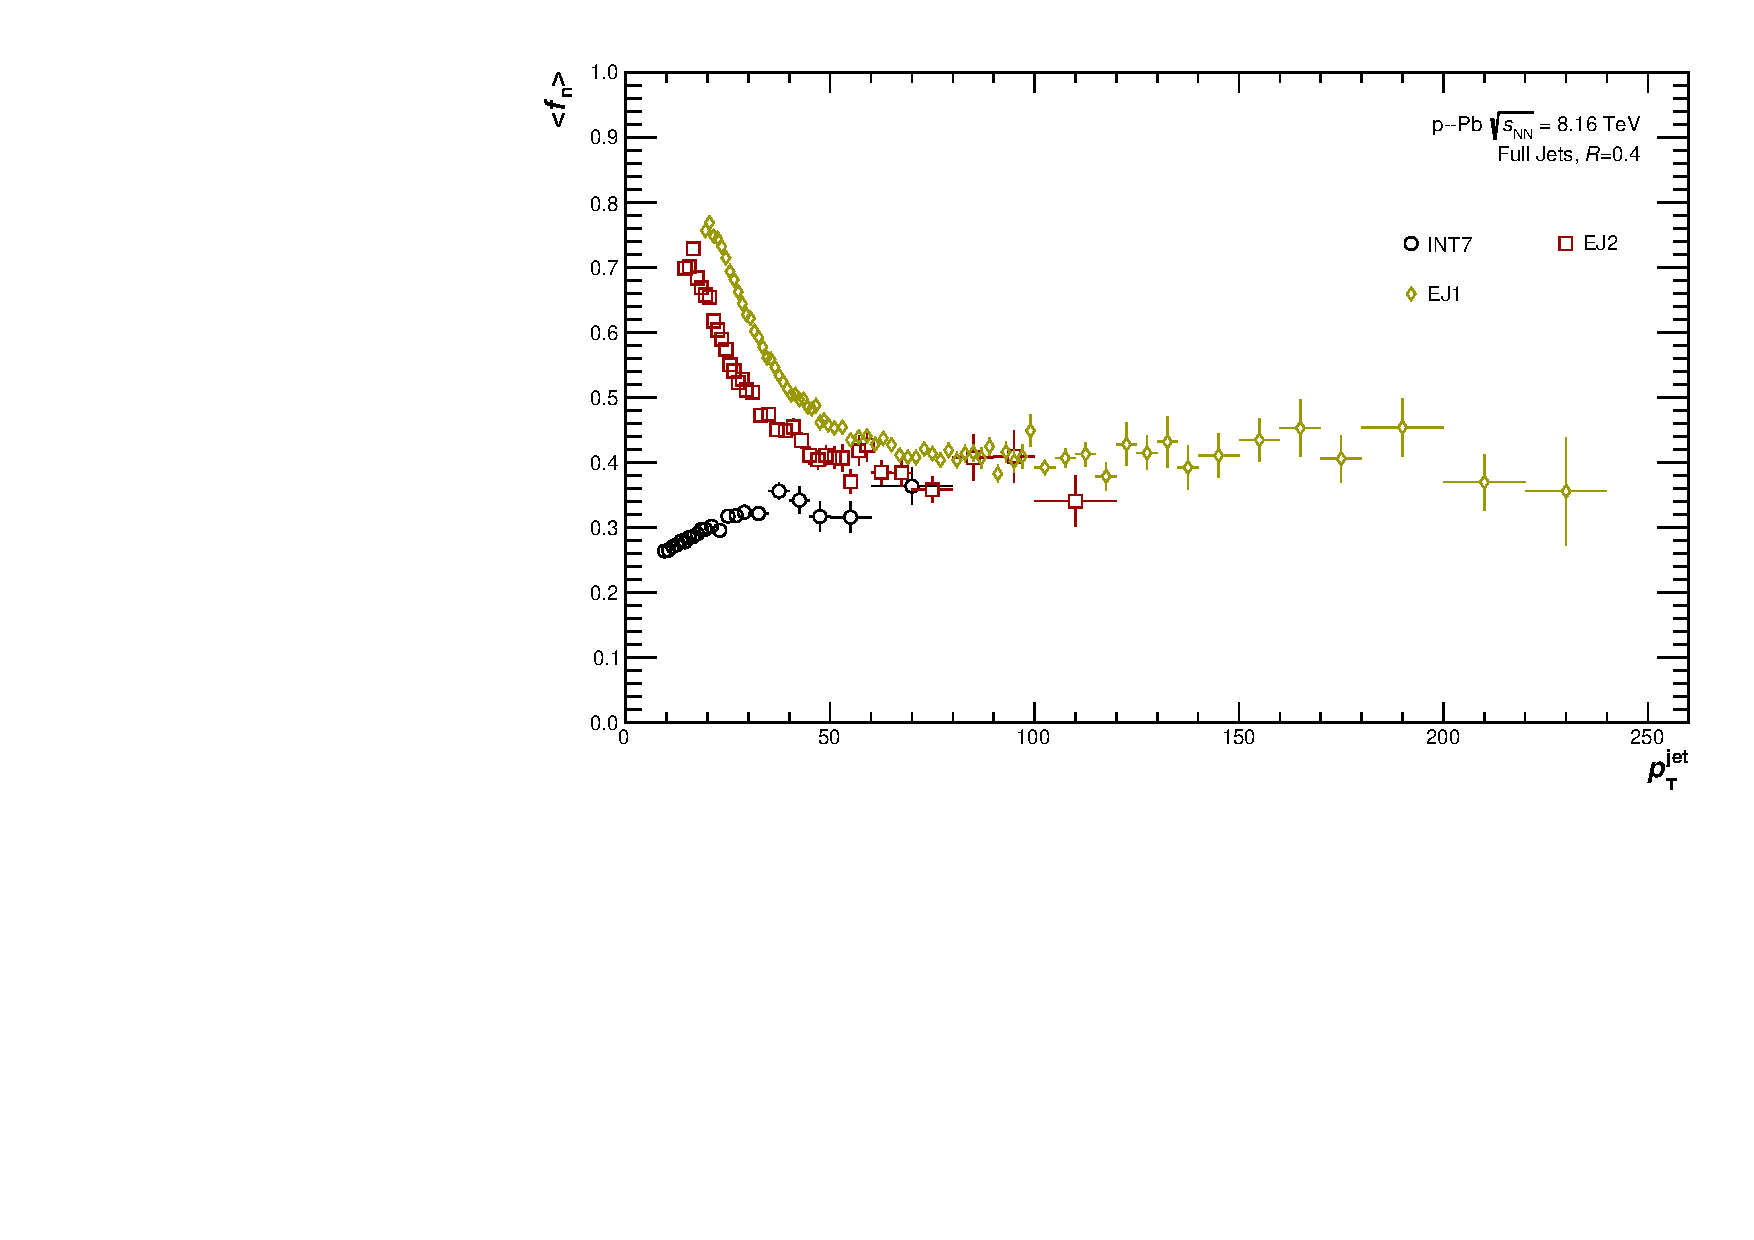
\includegraphics[width=0.49\textwidth]{figures/pPbFigures/TriggerBias/NEF/All/mean_NEF_R04.pdf}
    \caption{Mean neutral energy fraction as a function of jet \pT for jets in \pPb collisions for minimum bias and EMCal triggers, presented for various jet resolution parameters.}
    \label{fig:meanNEF_pPb}
\end{figure}

\begin{figure}[hbt!]
    \centering
    \begin{multicols}{2}
            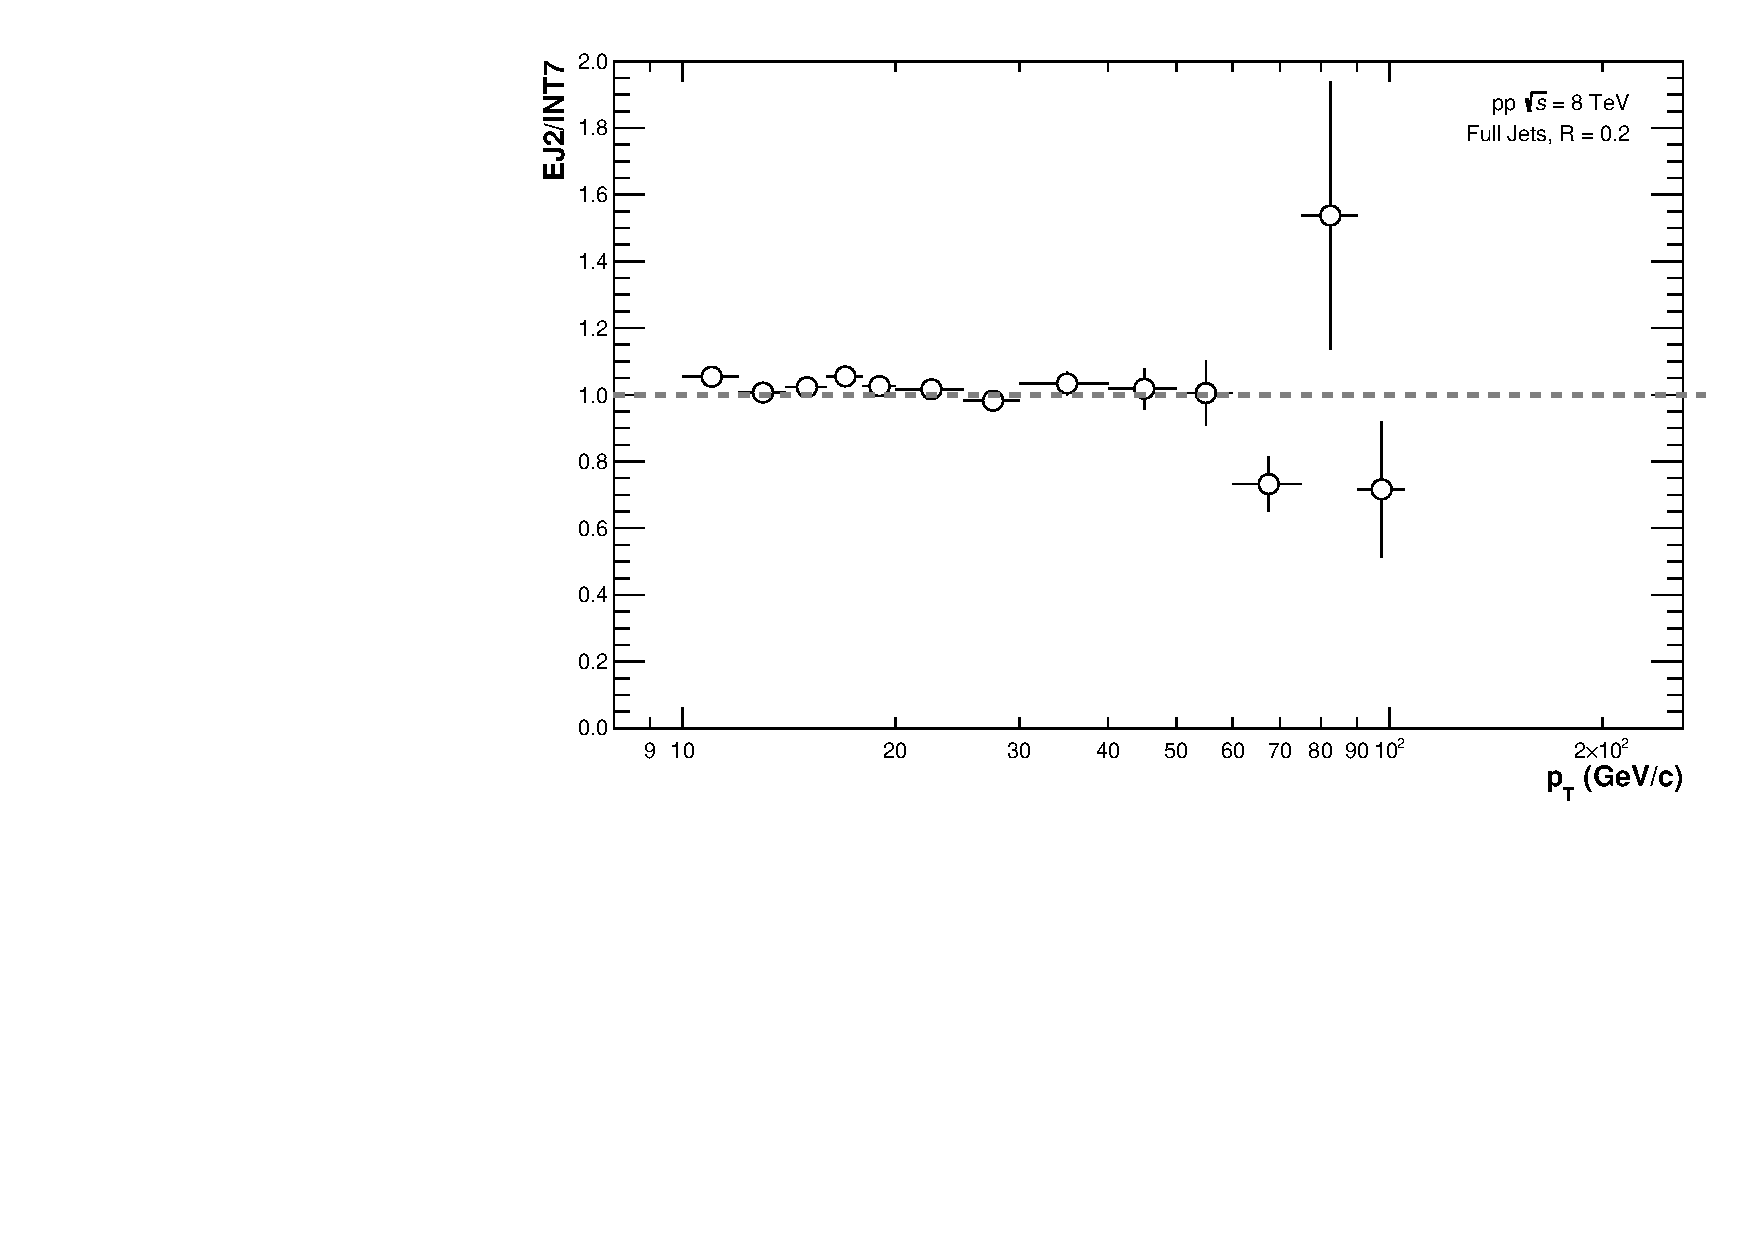
\includegraphics[width=0.49\textwidth]{figures/TriggerSwap/ratio_EMCINT_data_R02.pdf}
        \vfill\null 
        \columnbreak
            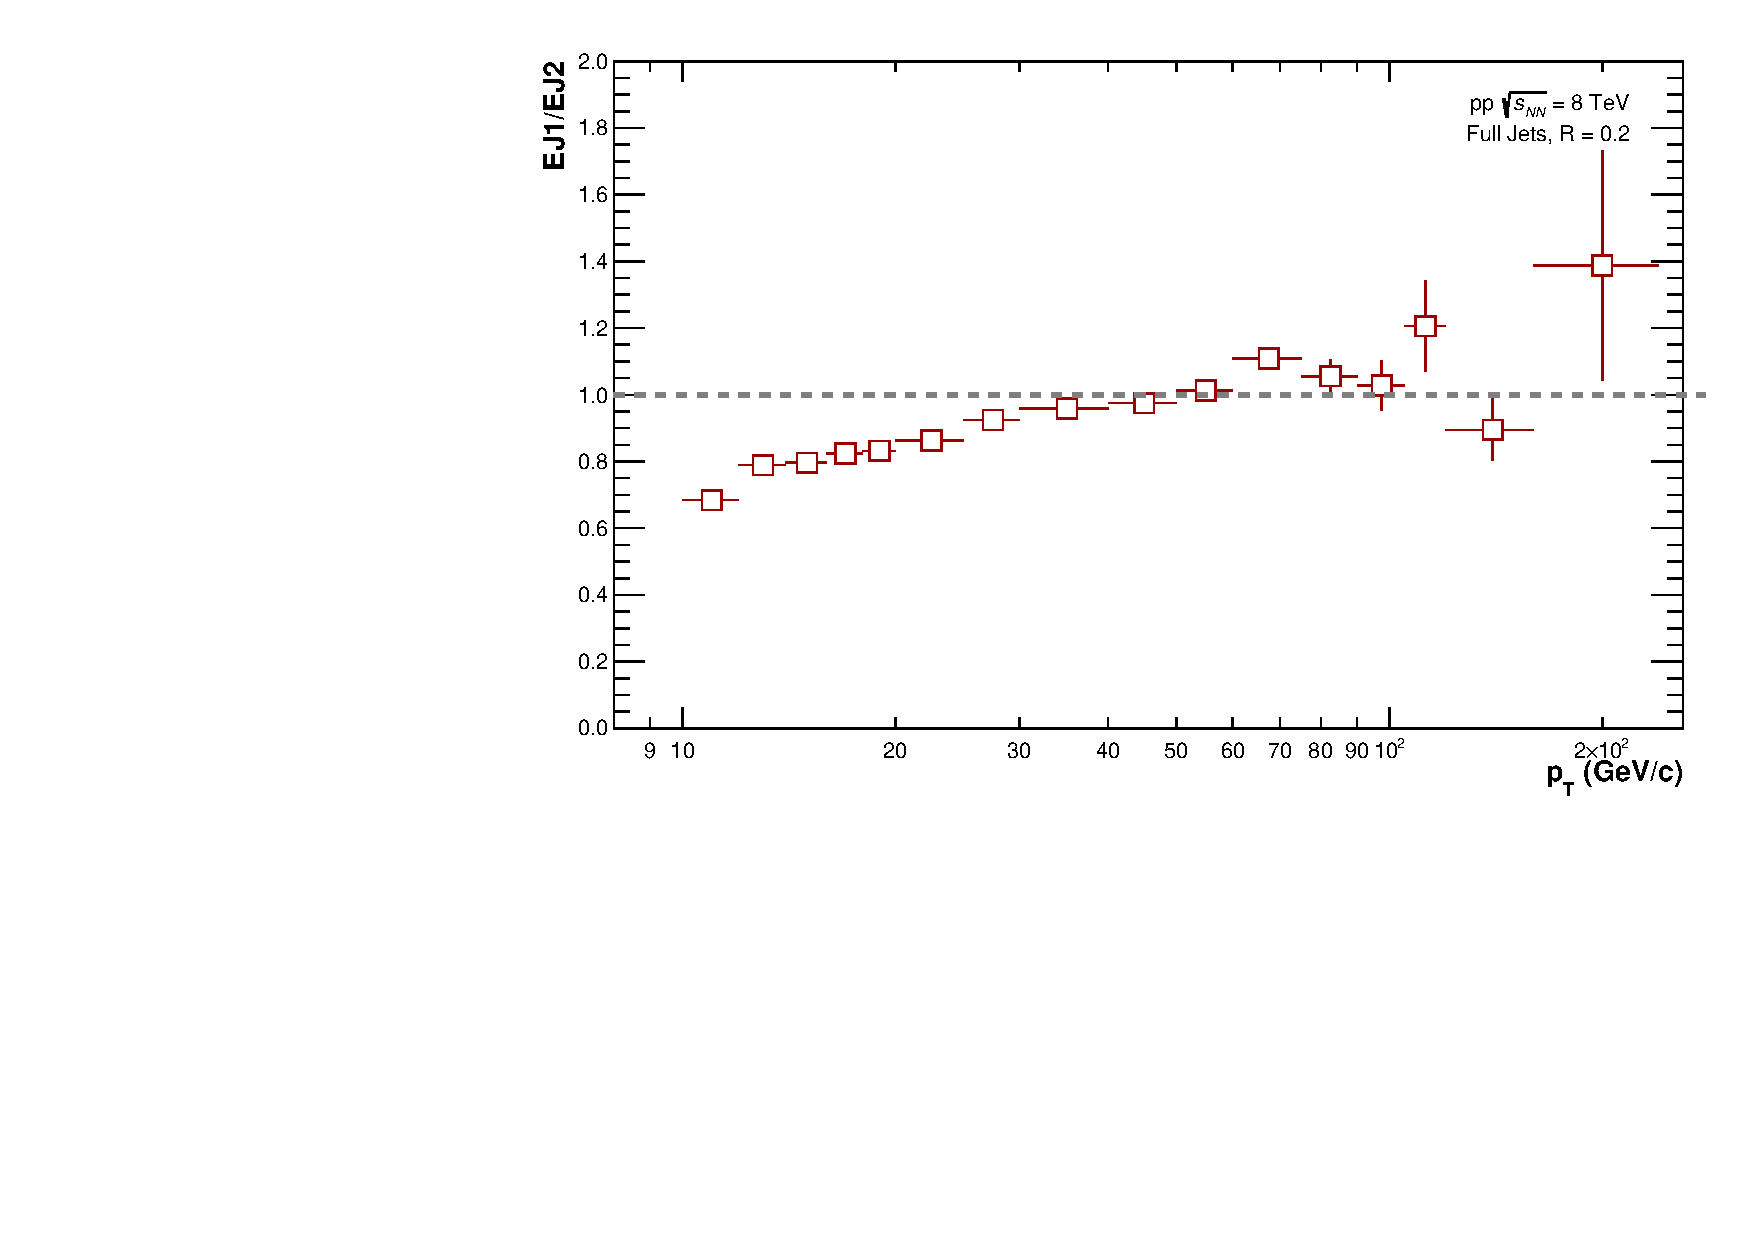
\includegraphics[width=0.49\textwidth]{figures/TriggerSwap/ratio_EJEEMC_data_R02.pdf}
        \vfill\null
    \end{multicols}
    \caption{Ratios of jet yield in \pp data of EMC7/INT7 triggers (left) and EJE/EMC7 triggers (right) as a function of jet \pT.}
    \label{fig:trigger_ratios}
\end{figure}

The trigger response in simulations is obtained by applying the same sliding window algorithm as implemented in the trigger hardware. The trigger uses the raw signal instead of the calibrated signal. Triggered events are required to have at least one trigger patch above the nominal threshold. The accuracy of the trigger bias in simulation is tested by comparing the distributions of the neutral energy fraction, z$_\mathrm{ch}$, and z$_\mathrm{neutral}$ between data and simulation. The observables z$_\mathrm{ch}$ and z$_\mathrm{neutral}$ are the fraction of the jet \pT coming from charged tracks and EMCal clusters. Figure~\ref{fig:TriggerBiasNEFR02} shows the comparison of the neutral energy fraction for jets from \pp collisions with R=0.2 in triggered events between data and simulations for different bins in \pT. The distributions obtained from simulation agree with the distributions obtained from data. 

Figure~\ref{fig:TriggerEfficiency_pp} shows the trigger efficiency for jets with resolution parameter $R$ = 0.2 to 0.5, obtained by taking the ratio of triggered jet spectra to minimum bias jet spectra in simulations of \pp collisions. The trigger becomes fully efficient before reaching the desired ranges of 30 GeV for EMC7 and 60 GeV for EJE. Figure~\ref{fig:TriggerEfficiency_pPb} shows the same in \pPb collisions for jets with resolution parameter $R$ = 0.2 to 0.4. The trigger efficiency never reaches unity but instead plateaus at about 99\% in \pp and about 90\% in \pPb. This is due to the masking of channels at trigger level that are not masked in the front-end readout electronics. Since masking in the front-end electronics is performed at L0, the acceptance is the same for both L0 and L1 trigger levels. Additionally, there are contributions from jets which contain only particles that are never reconstructed, such as $K_L^0$, and from jets that never get matched due to the finite matching efficiency. In the low momentum region, other detector effects which are not simulated (i.e. random noise) play a role and the simulated trigger efficiency will overestimate the correction.


\begin{figure}[hbt!]
    \centering
    \begin{multicols}{2}
            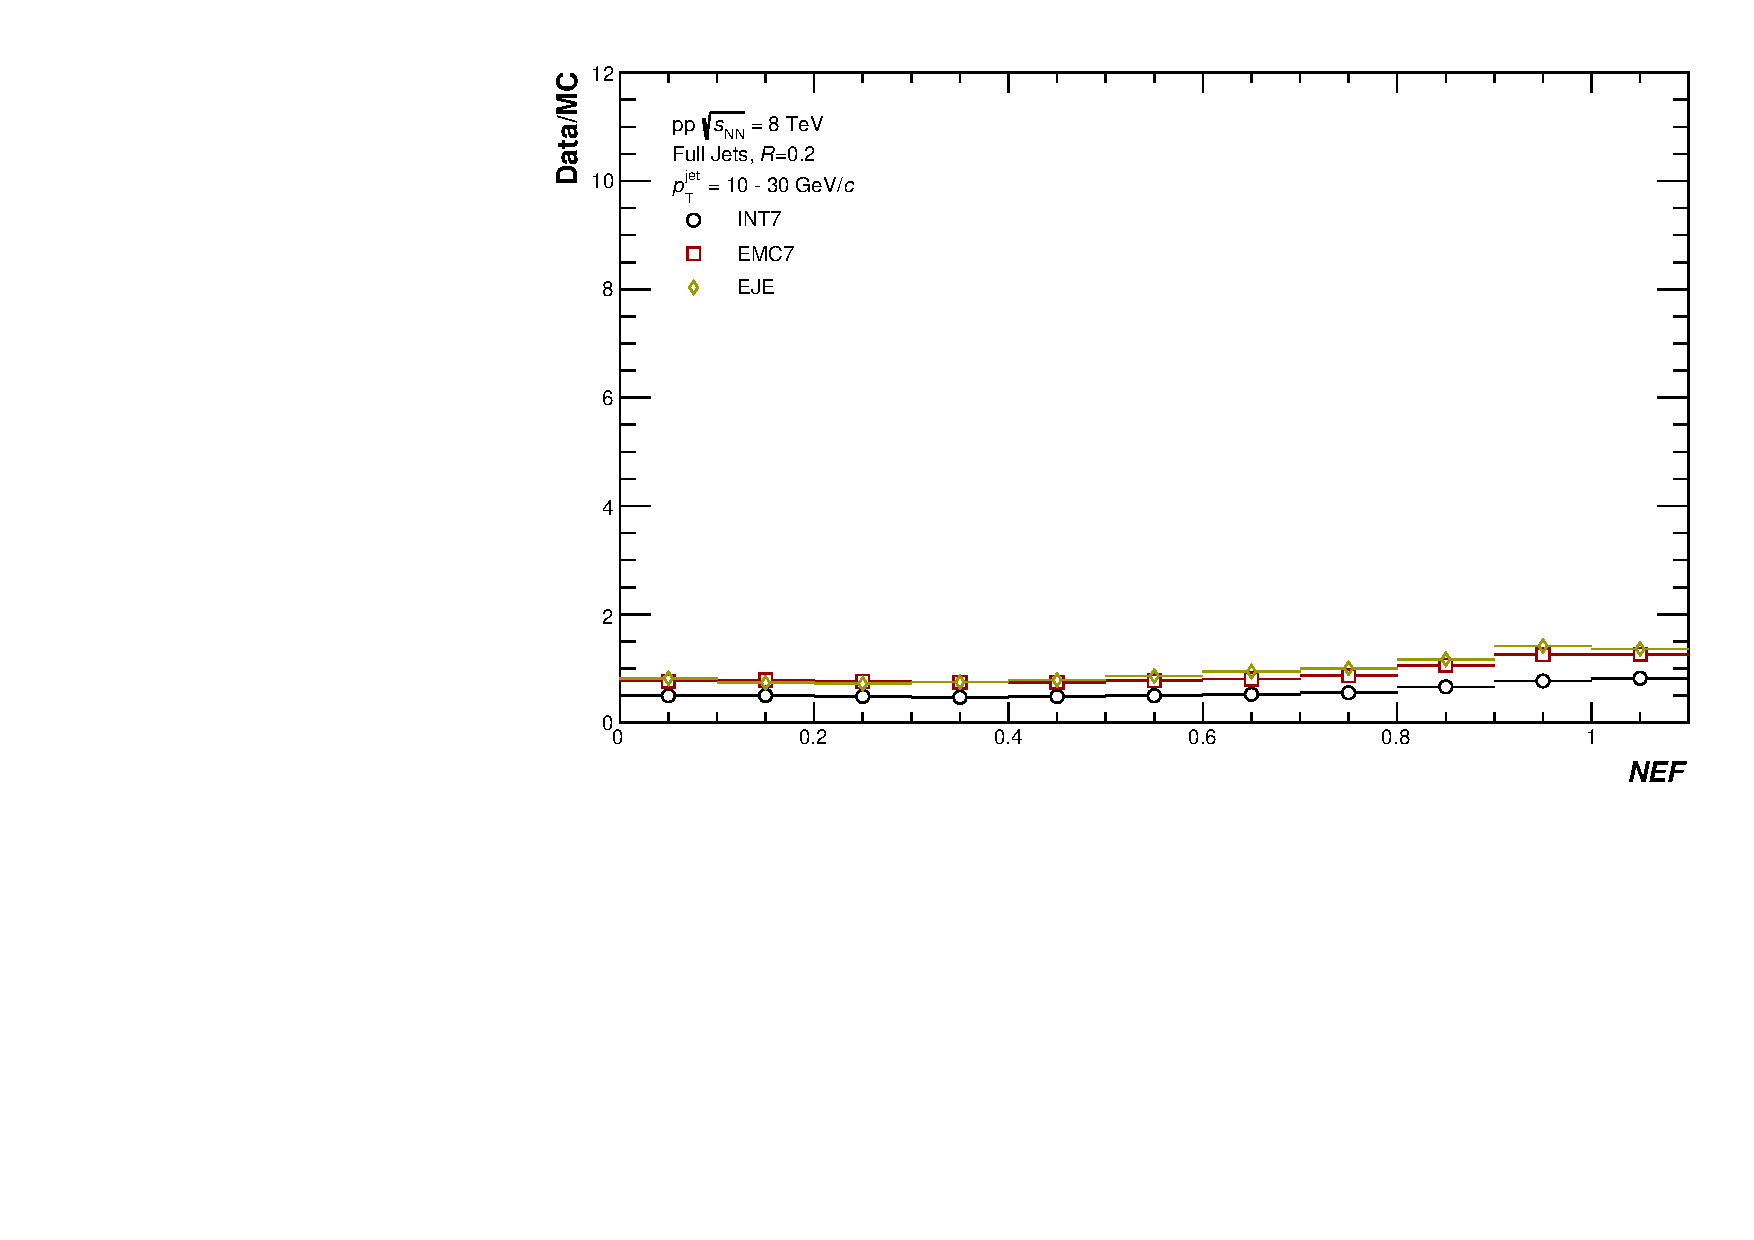
\includegraphics[width=0.49\textwidth]{figures/TriggerBias/NEF/hNEF_ptBin1_R02.pdf}
            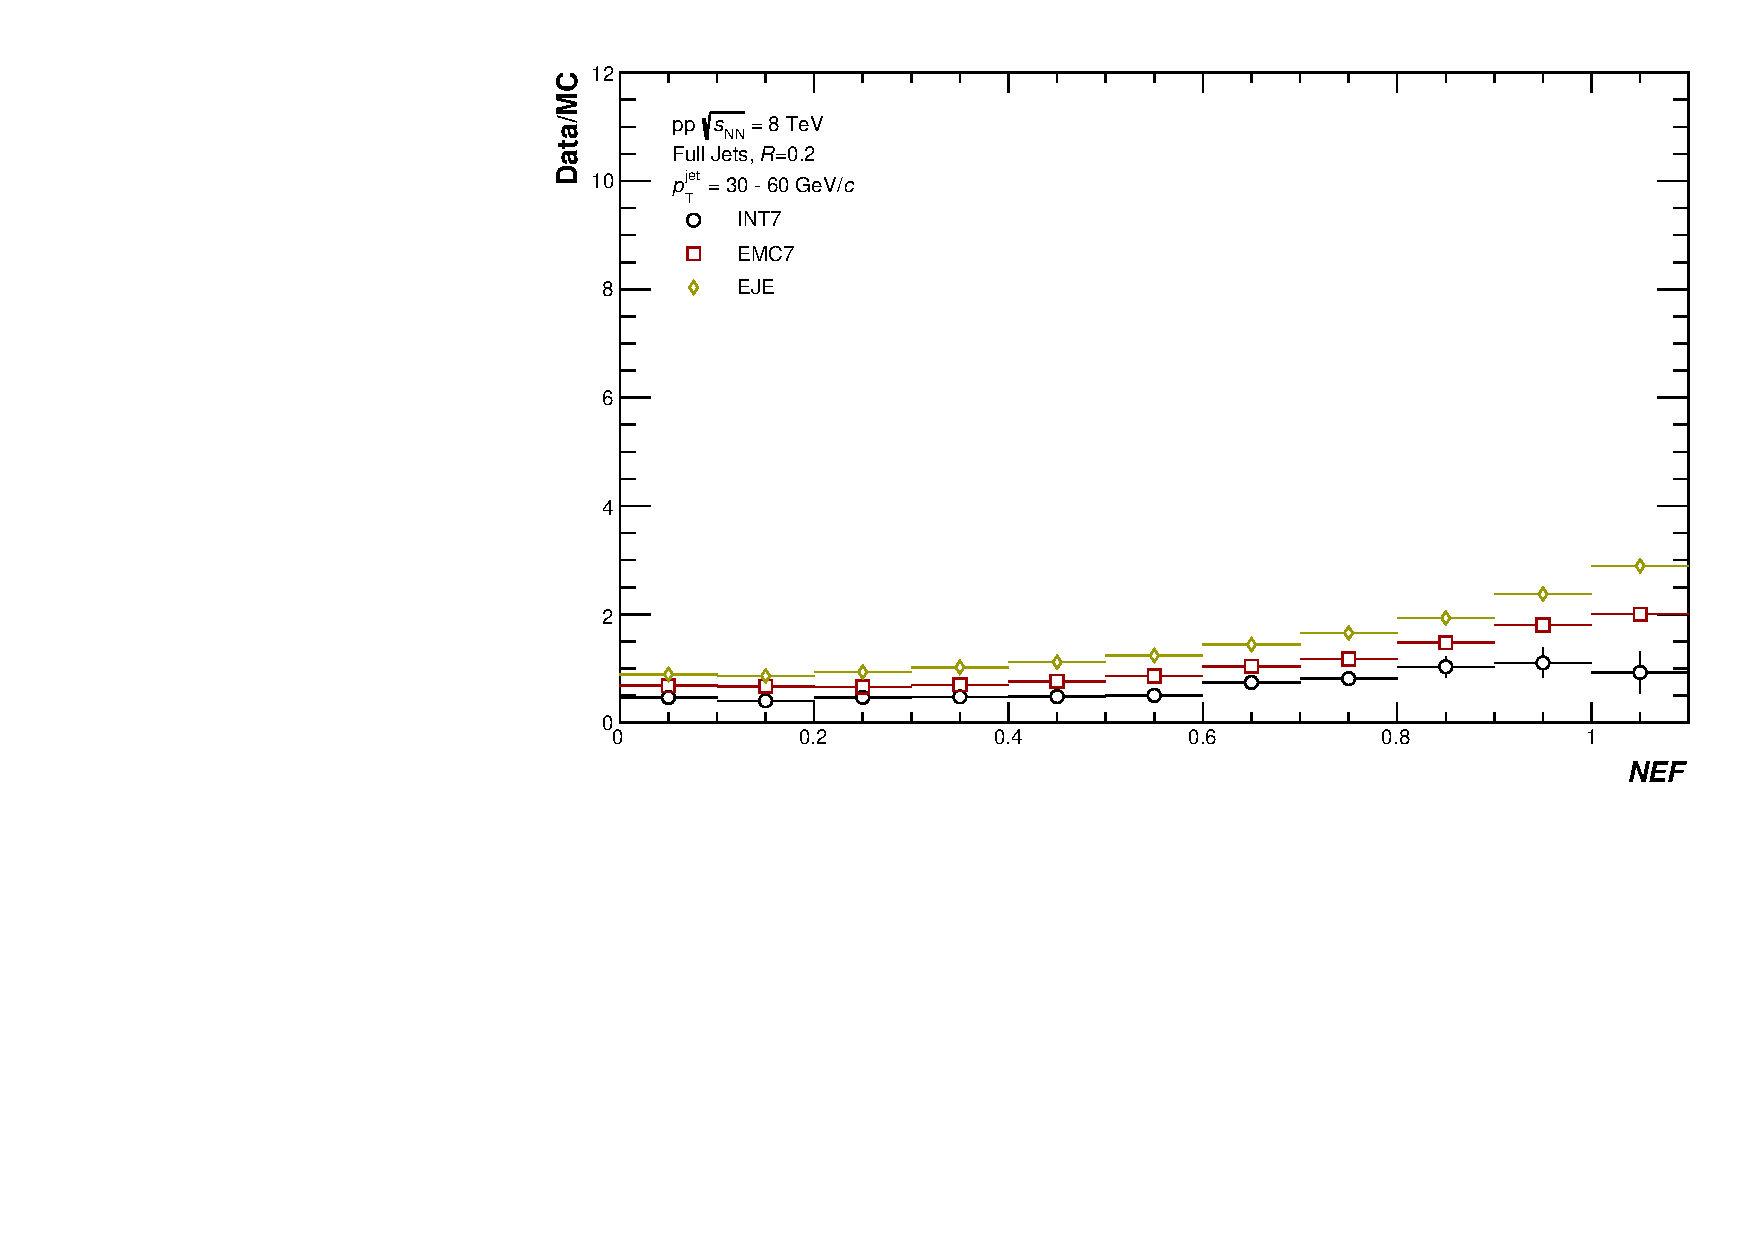
\includegraphics[width=0.49\textwidth]{figures/TriggerBias/NEF/hNEF_ptBin2_R02.pdf}
        \vfill\null
        \columnbreak
            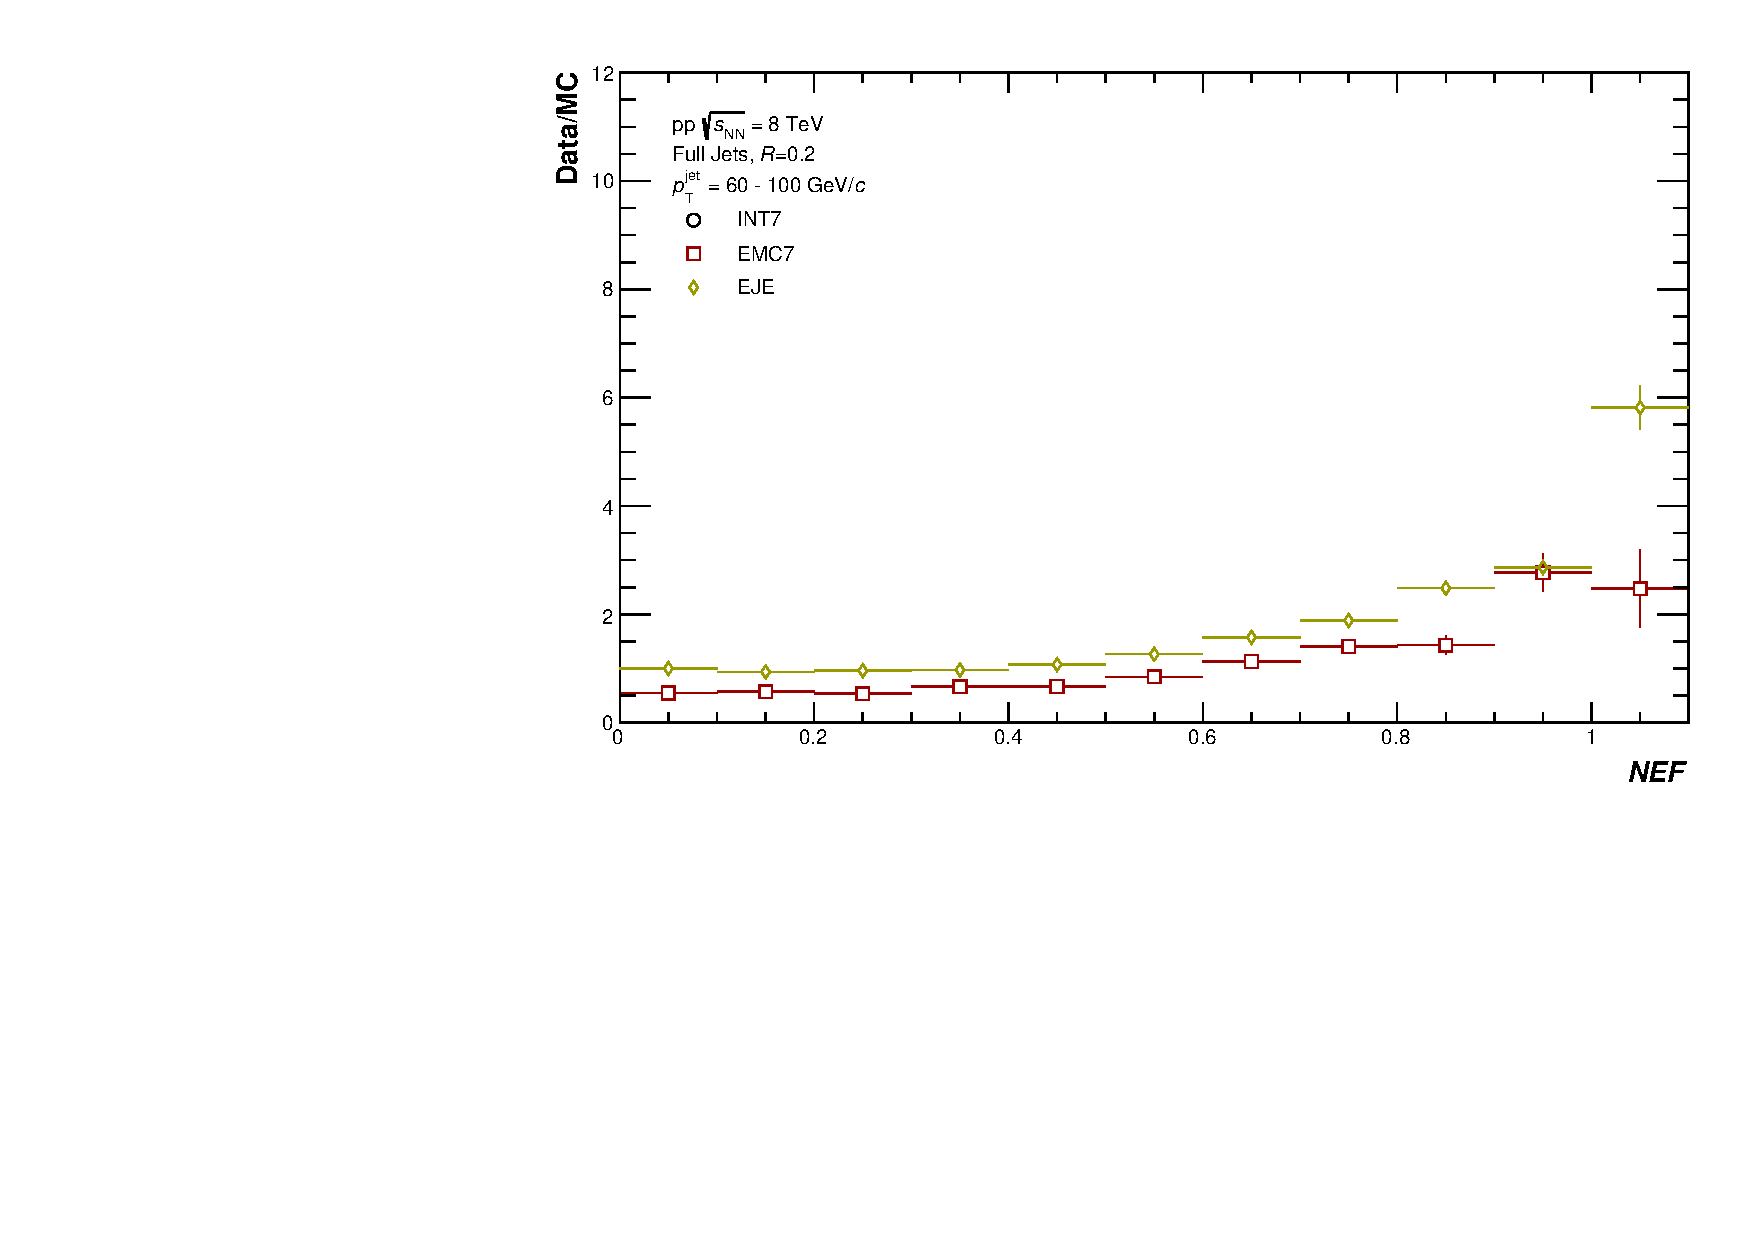
\includegraphics[width=0.49\textwidth]{figures/TriggerBias/NEF/hNEF_ptBin3_R02.pdf}
            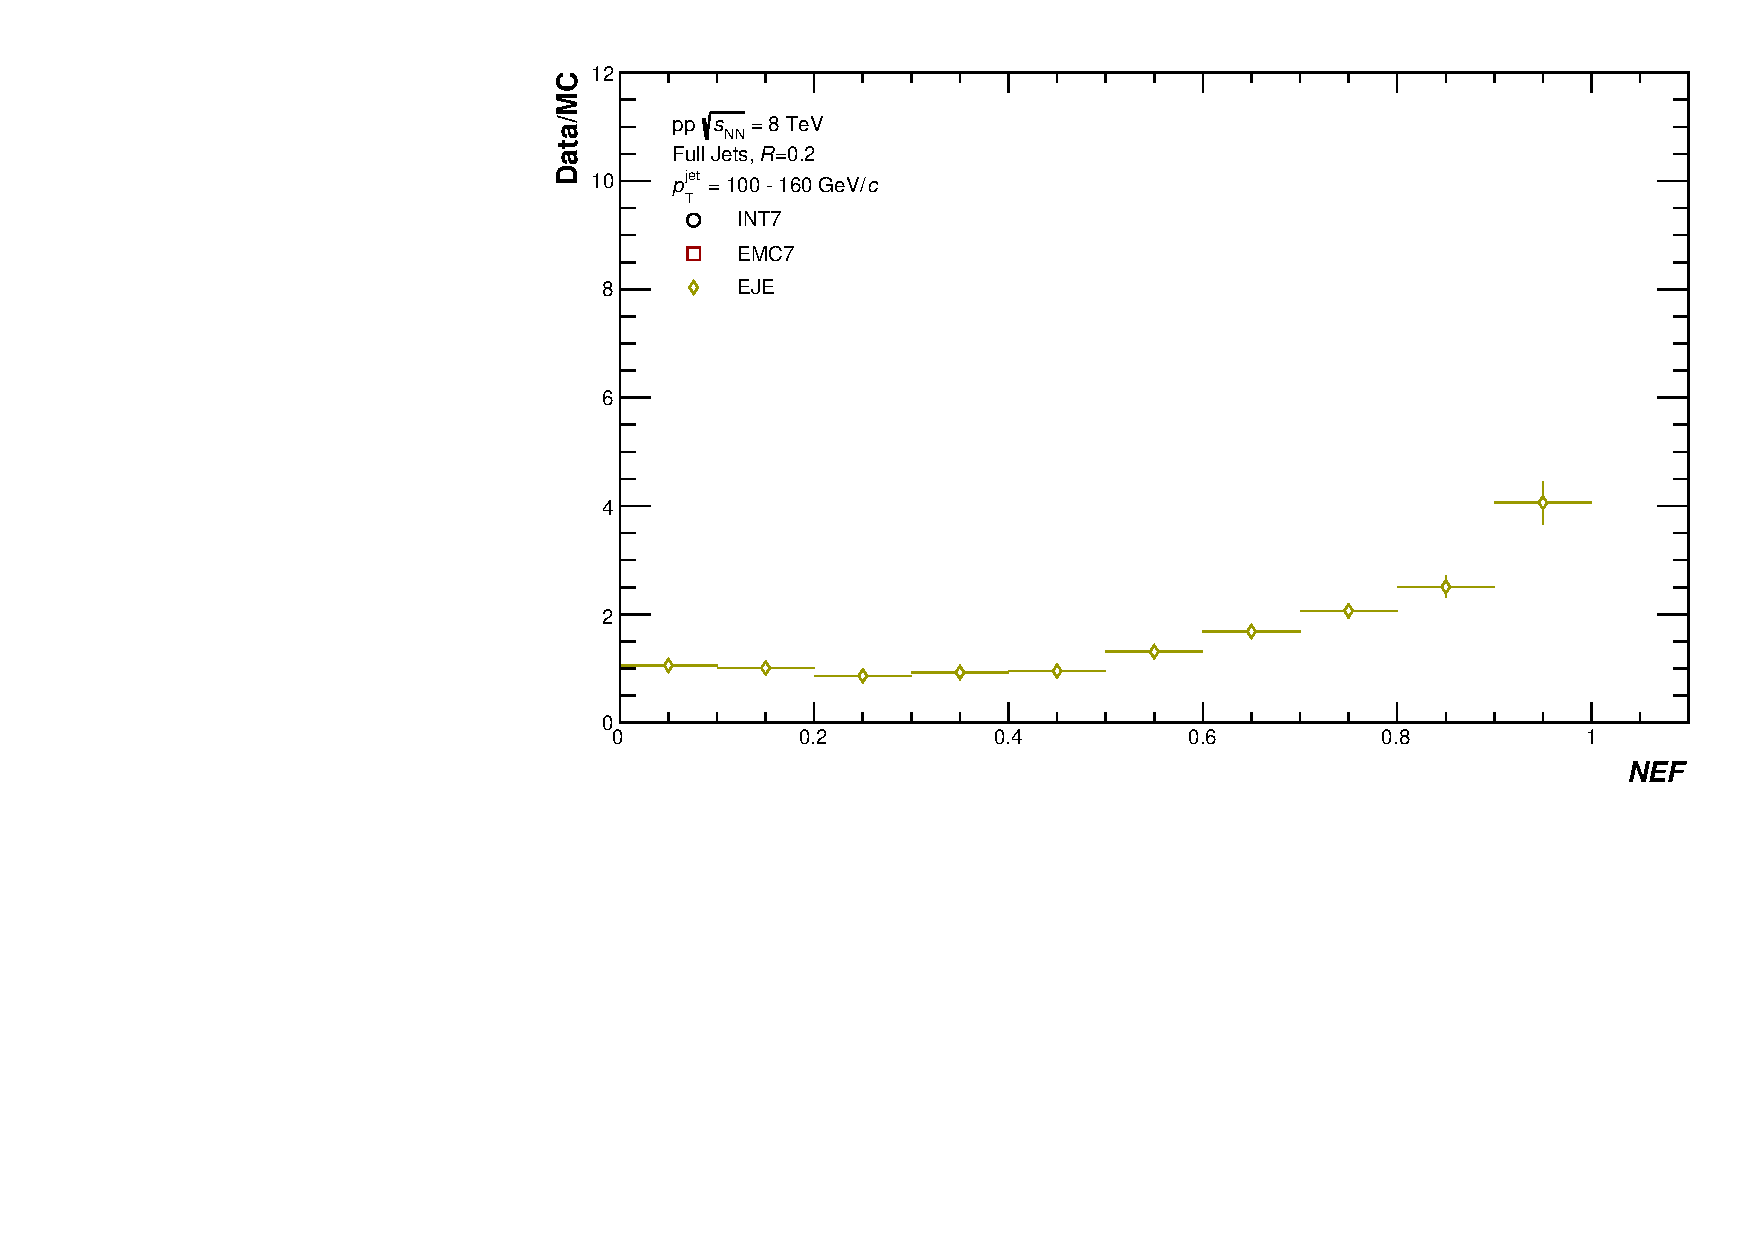
\includegraphics[width=0.49\textwidth]{figures/TriggerBias/NEF/hNEF_ptBin4_R02.pdf}
        \vfill\null
    \end{multicols}
    \caption{neutral energy fraction ratios of \pp data to Monte Carlo for different bins in jet \pT and a jet resolution parameter of R=0.2.}
    \label{fig:TriggerBiasNEFR02}
\end{figure}

\begin{figure}[hbt!]
    \centering
    \begin{multicols}{2}
            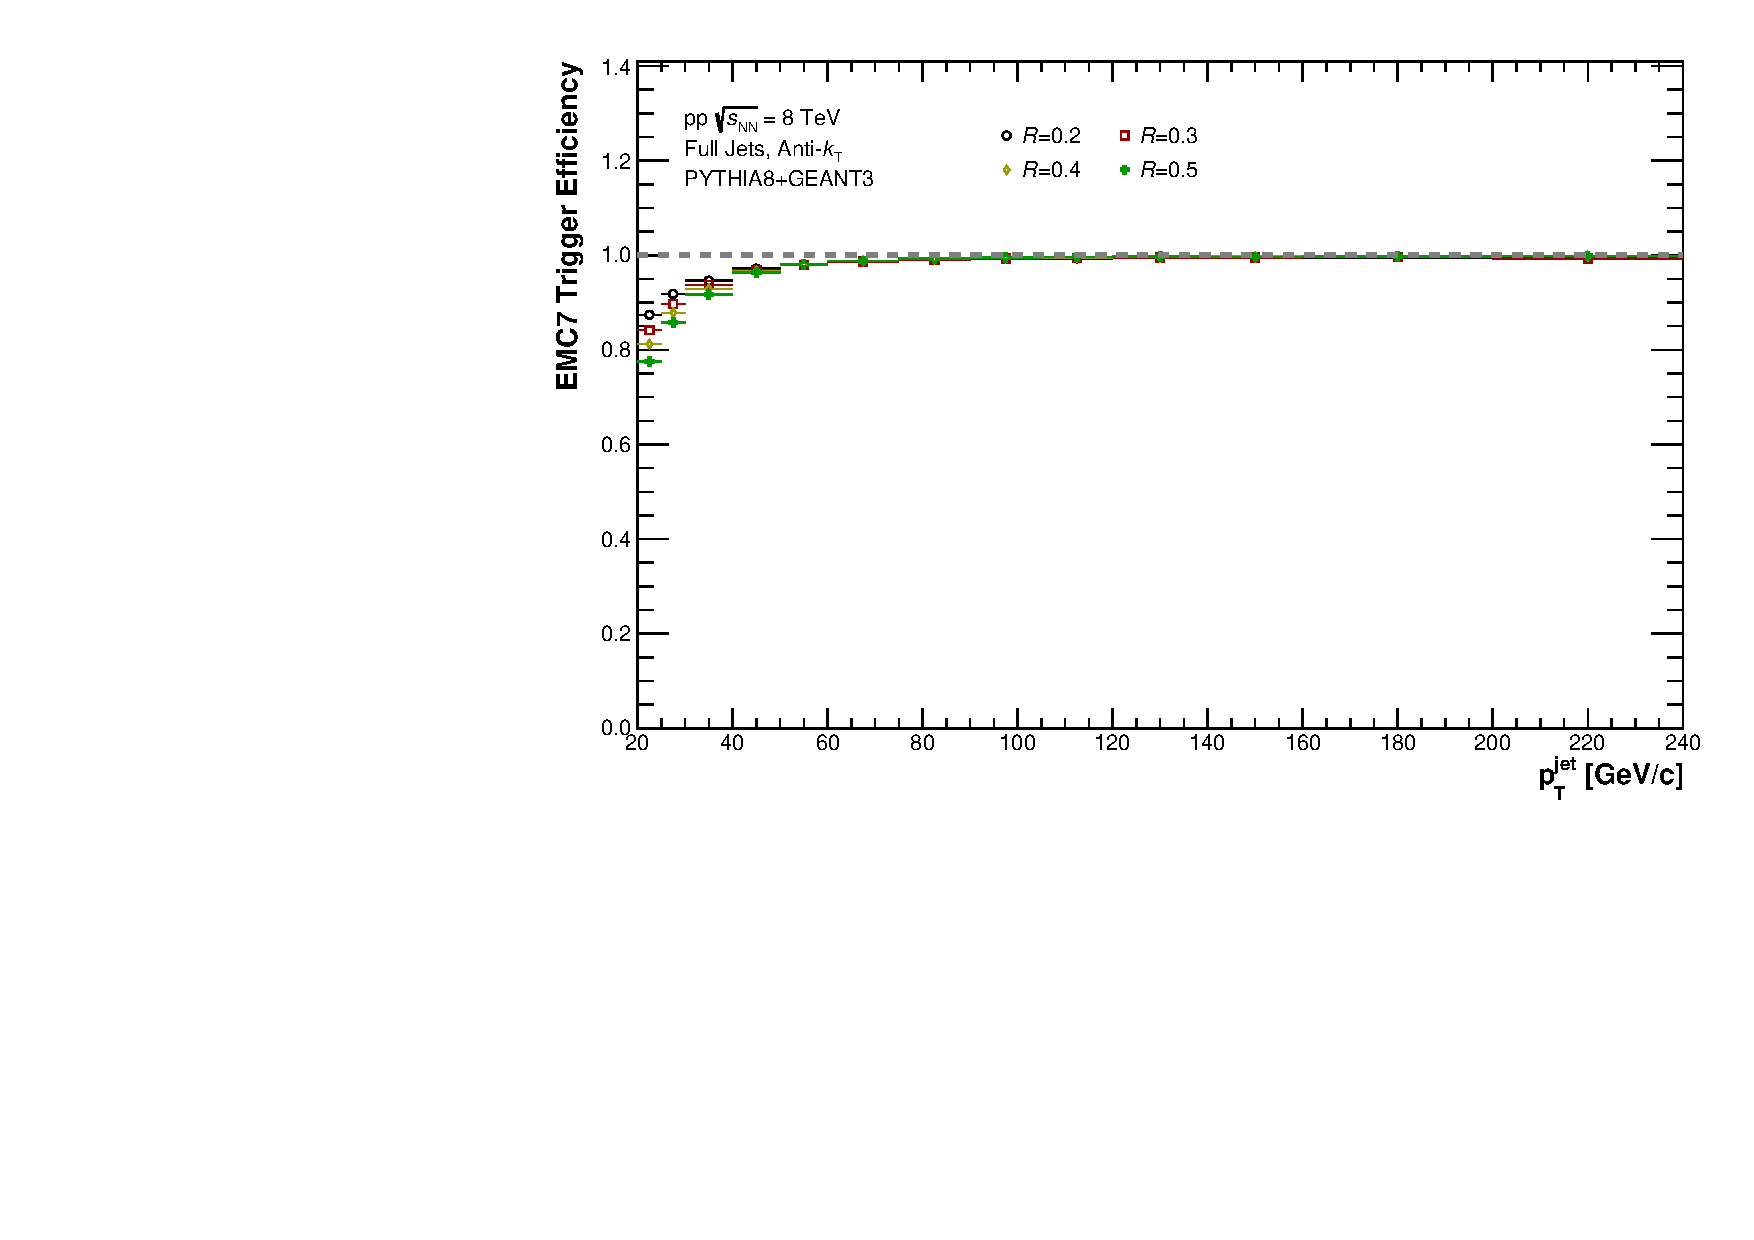
\includegraphics[width=0.49\textwidth]{figures/TriggerEfficiency/hEfficiency_EMC7.pdf}
        \vfill\null
        \columnbreak
            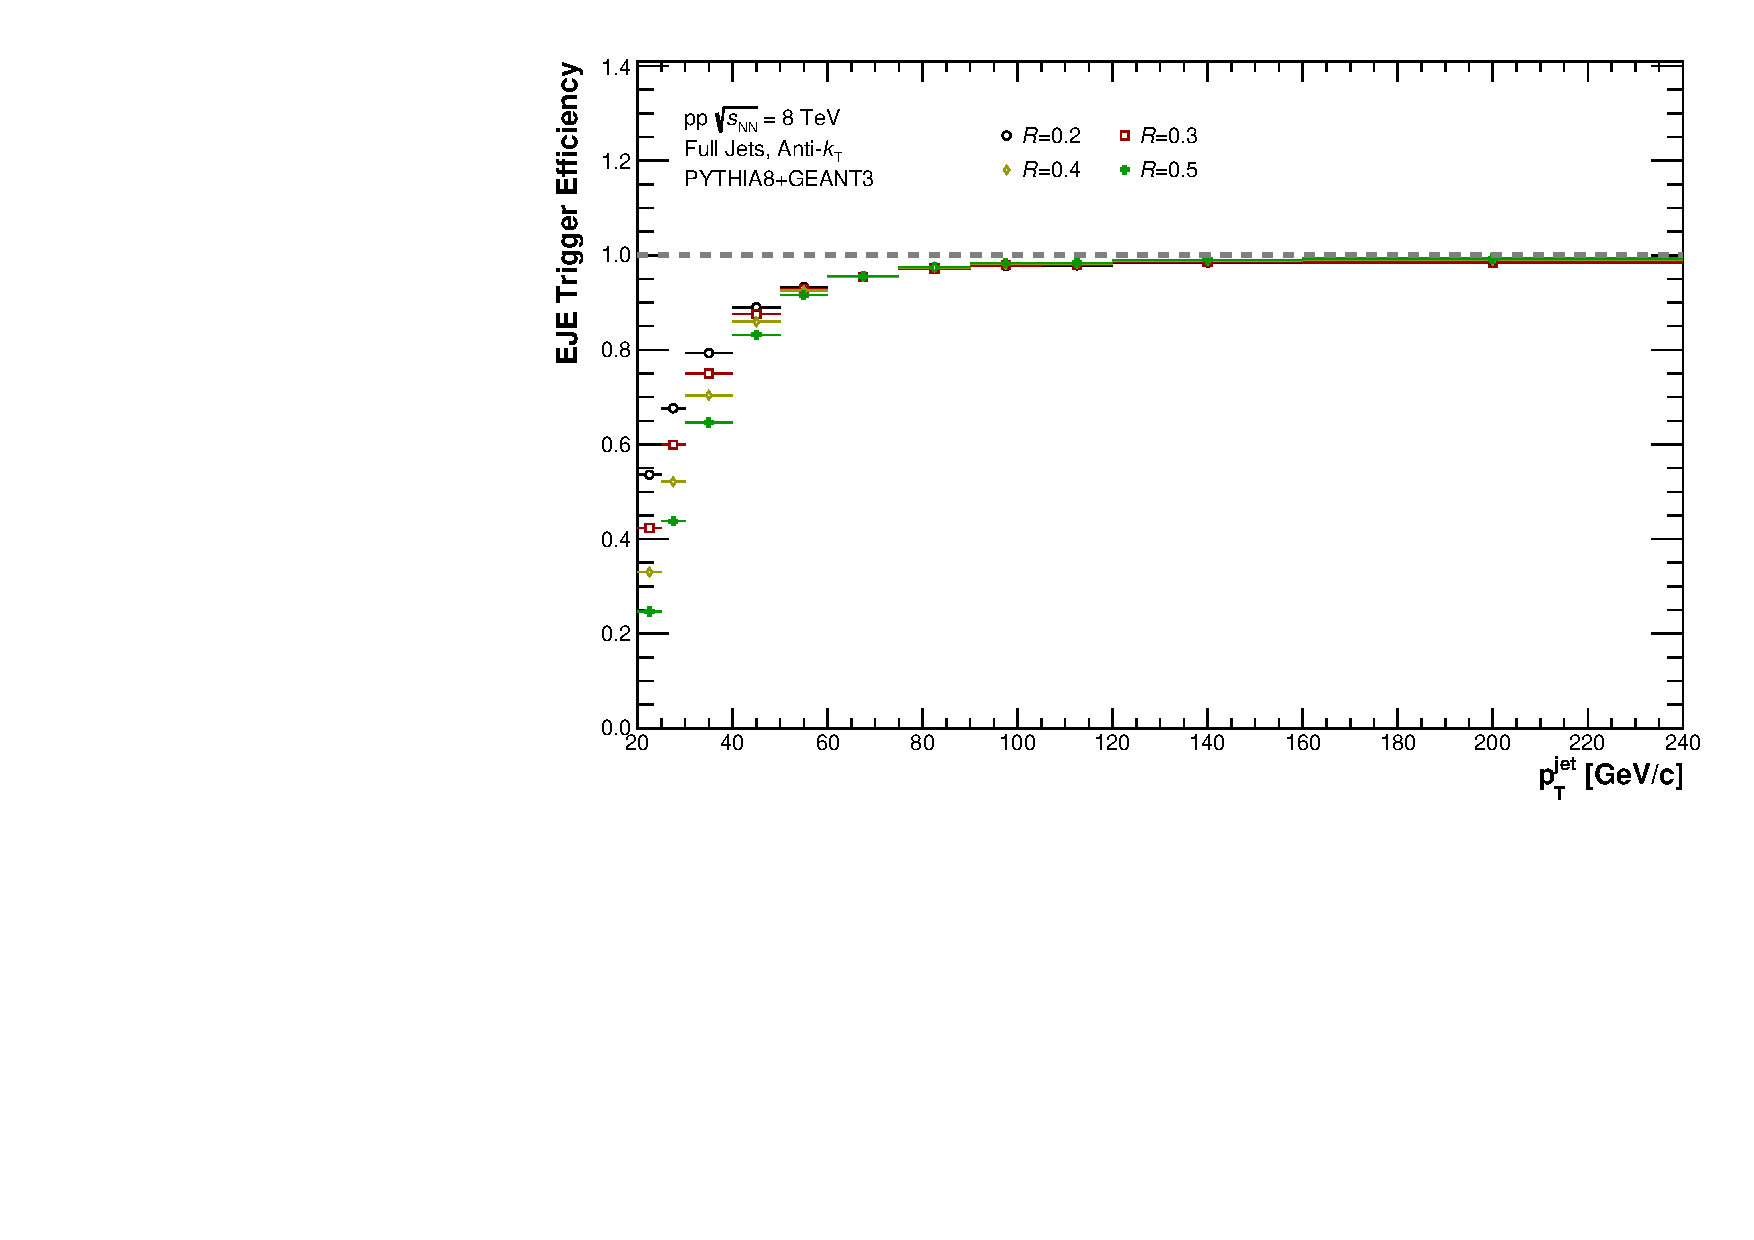
\includegraphics[width=0.49\textwidth]{figures/TriggerEfficiency/hEfficiency_EJE.pdf}
        \vfill\null
    \end{multicols}
    \caption{Trigger efficiency for the EMC7 trigger (left) and the EJE trigger (right), found by taking the ratio of trigger/minimum bias in \pp simulation.}
    \label{fig:TriggerEfficiency_pp}
\end{figure}

\begin{figure}[hbt!]
    \centering
    \begin{multicols}{2}
            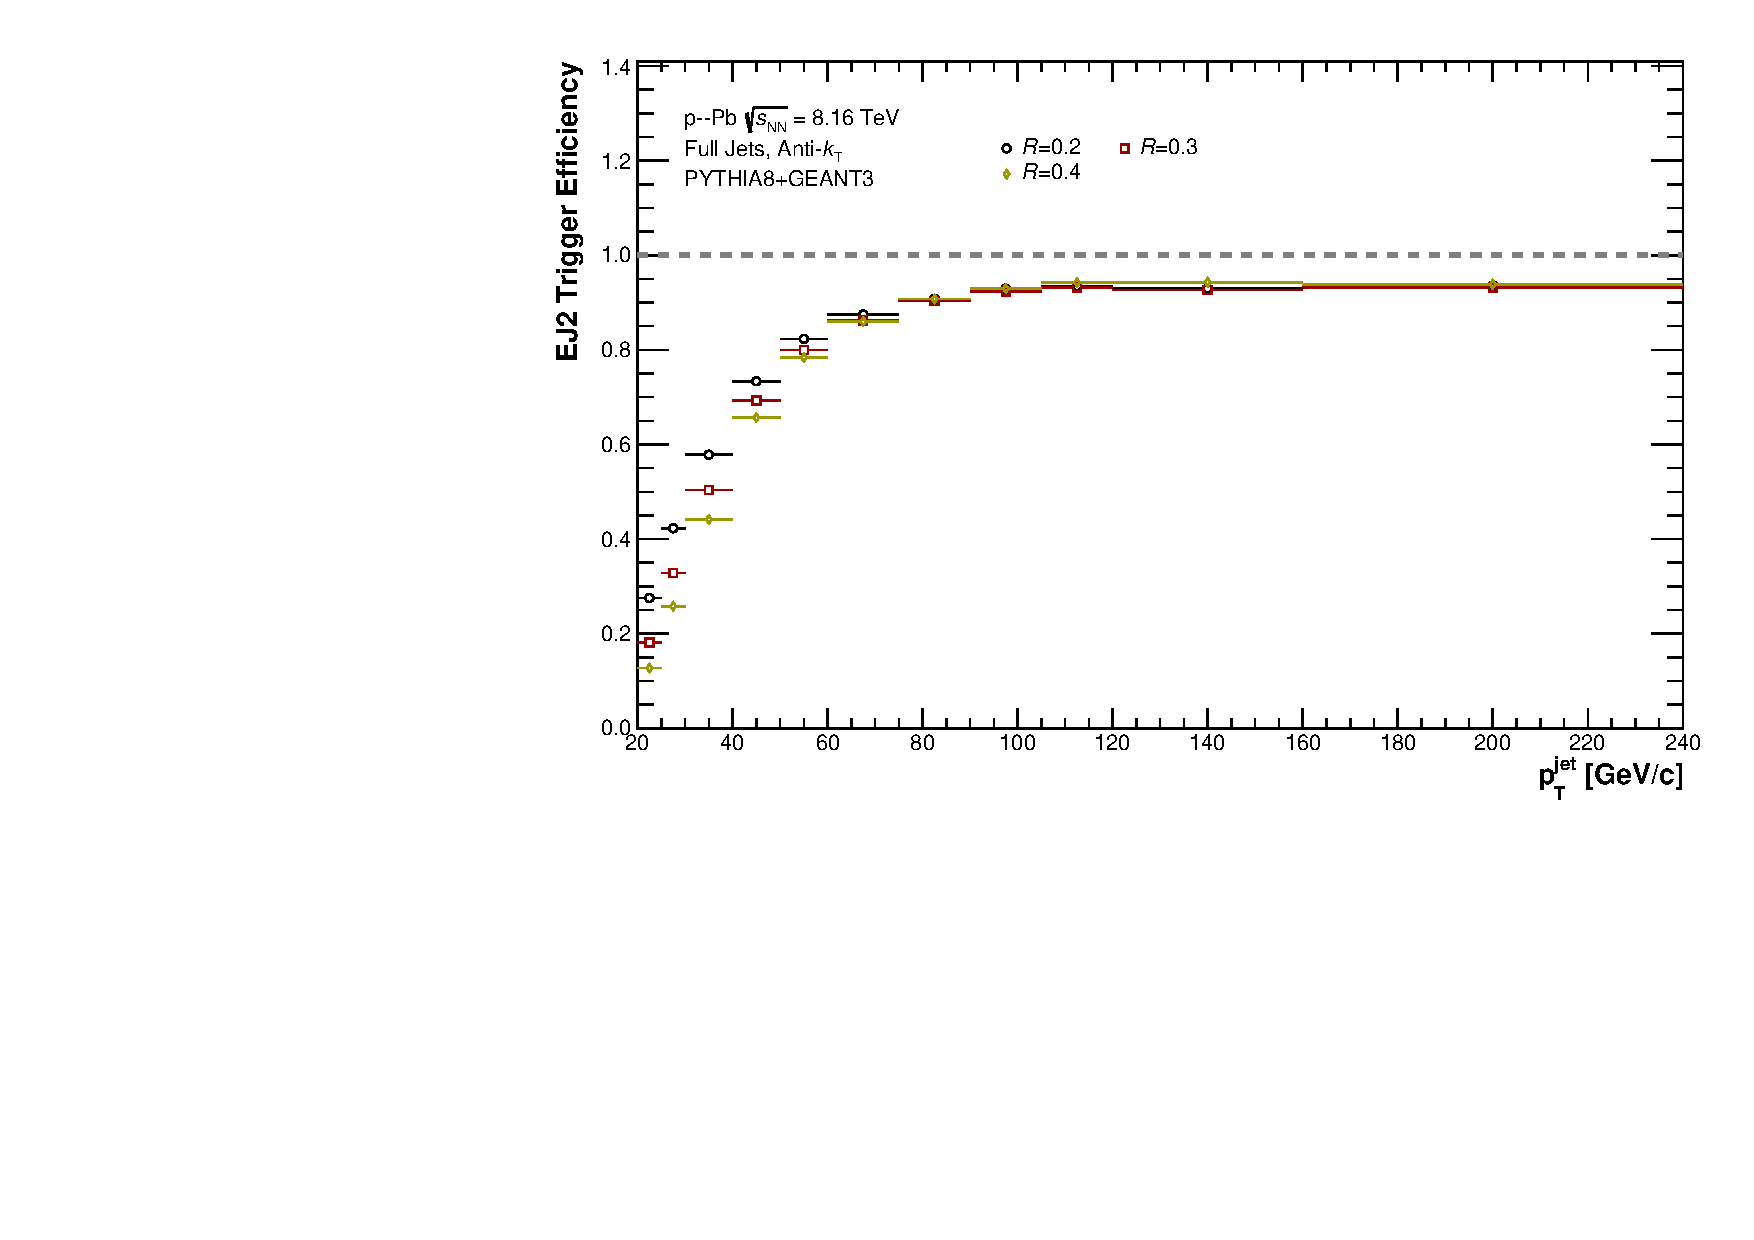
\includegraphics[width=0.49\textwidth]{figures/pPbFigures/TriggerEfficiency/hEfficiency_EJ2.pdf}
        \vfill\null
        \columnbreak
            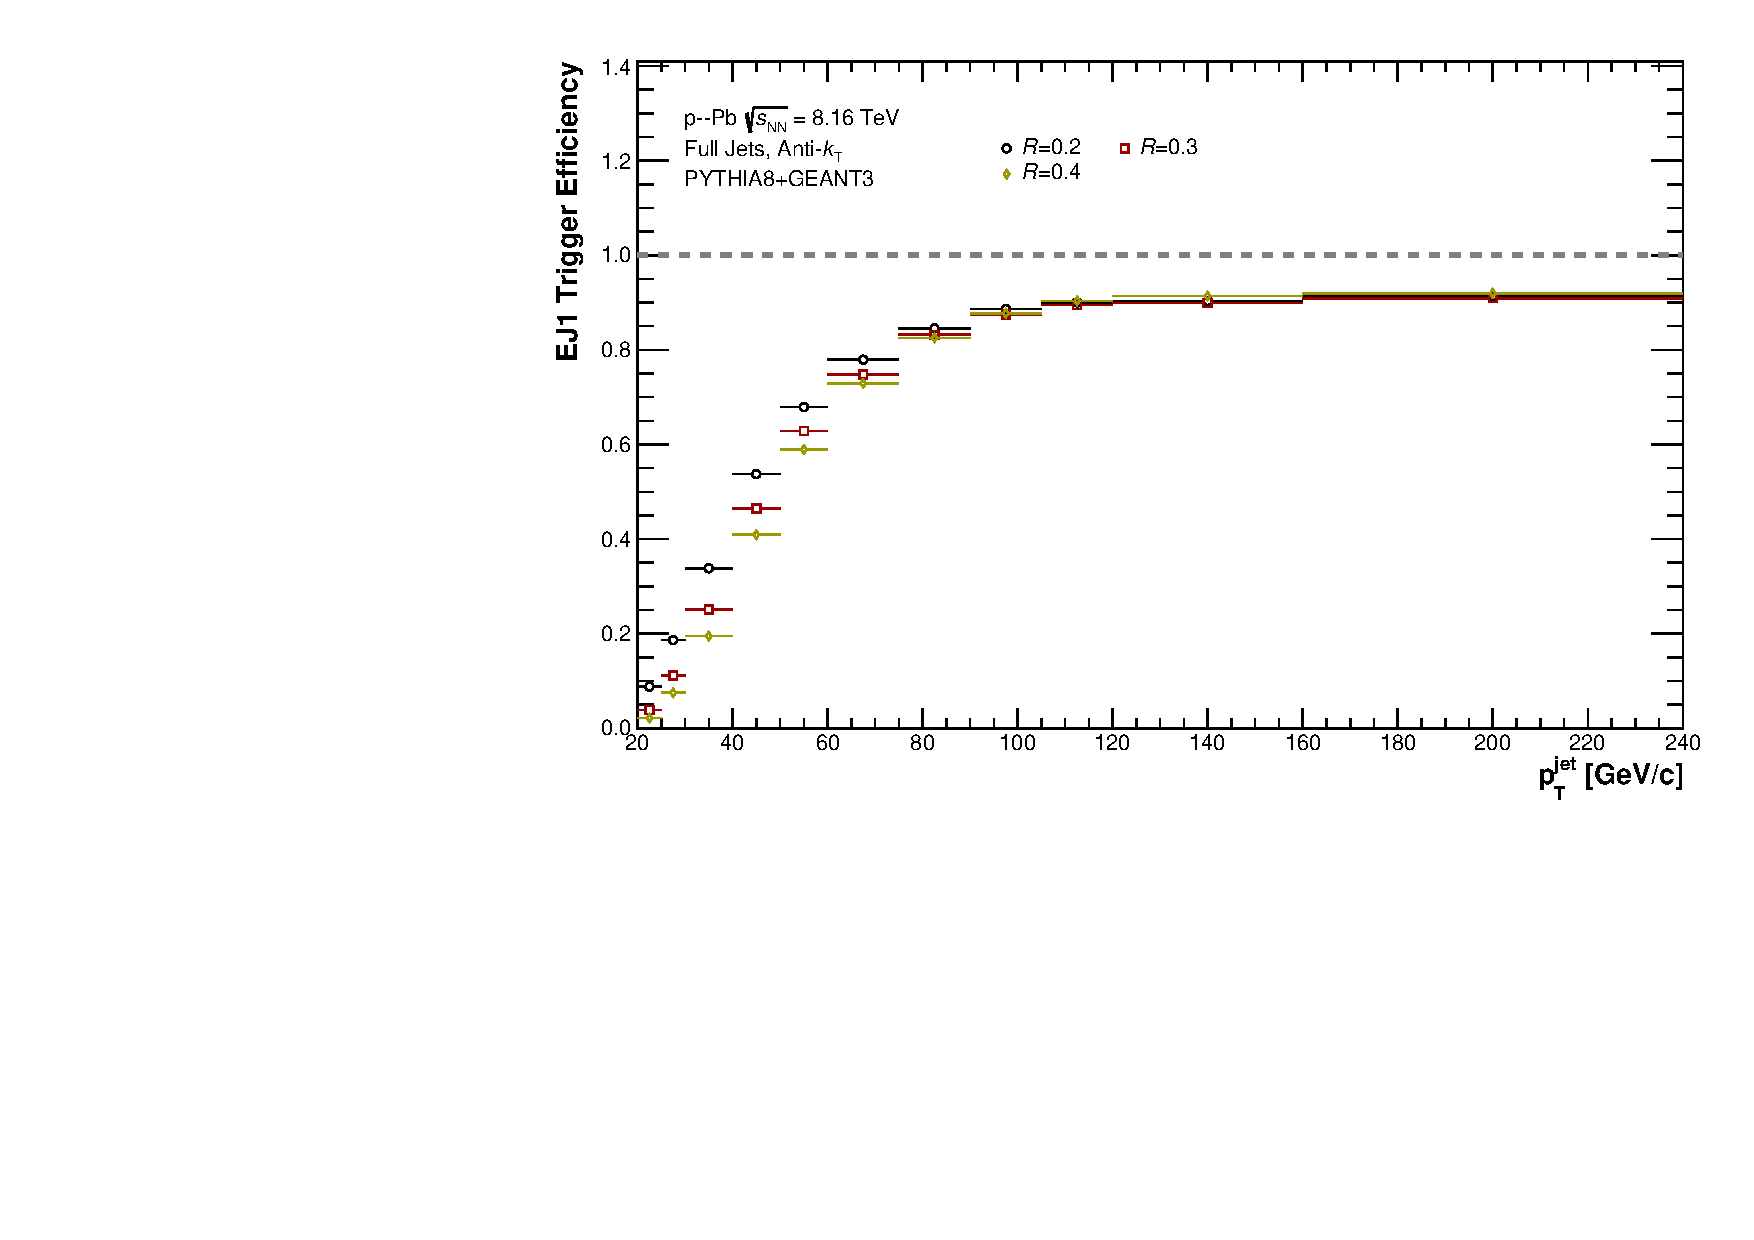
\includegraphics[width=0.49\textwidth]{figures/pPbFigures/TriggerEfficiency/hEfficiency_EJ1.pdf}
        \vfill\null
    \end{multicols}
    \caption{Trigger efficiency for the EJ2 trigger (left) and the EJ1 trigger (right), found by taking the ratio of trigger/minimum bias in \pPb simulation.}
    \label{fig:TriggerEfficiency_pPb}
\end{figure}